% !TEX TS-program = lualatex
% !TEX encoding = UTF-8 Unicode

\documentclass[12pt, letterpaper]{article}

%%BIBLIOGRAPHY- This uses biber/biblatex to generate bibliographies according to the 
%%Unified Style Sheet for Linguistics
\usepackage[main=american, german]{babel}% Recommended
\usepackage{csquotes}% Recommended
\usepackage[backend=biber,
             style=unified,
             maxcitenames=3,
             maxbibnames=99,
             natbib,
             url=false]{biblatex}
\addbibresource{Library.bib}
\setcounter{biburlnumpenalty}{100}  % allow URL breaks at numbers
%\setcounter{biburlucpenalty}{100}   % allow URL breaks at uppercase letters
%\setcounter{biburllcpenalty}{100}   % allow URL breaks at lowercase letters

%%TYPOLOGY
\usepackage[svgnames]{xcolor} % Specify colors by their 'svgnames', for a full list of all colors available see here: http://www.latextemplates.com/svgnames-colors
%\usepackage[compact]{titlesec}
%\titleformat{\section}[runin]{\normalfont\bfseries}{\thesection.}{.5em}{}[.]
%\titleformat{\subsection}[runin]{\normalfont\scshape}{\thesubsection}{.5em}{}[.]
\usepackage[hmargin=1in,vmargin=1in]{geometry}  %Margins
\usepackage{graphicx} % 
\usepackage{stackengine} %Package to allow text above or below other text, Also helpful for HG weights 
\usepackage{fontspec} %Selection of fonts must be ran in XeLaTeX
\usepackage{amssymb} %Math symbols
\usepackage{amsmath} % Mathematical enhancements for LaTeX
\usepackage{setspace} %Linespacing
\usepackage{multicol} %Multicolumn text
\usepackage{enumitem} %Allows for continuous numbering of lists over examples, etc.
\usepackage{multirow} %Useful for combining cells in tablesbrew 
\usepackage{booktabs}
\usepackage{hanging}
\usepackage{fancyhdr} %Allows for the 
\pagestyle{fancy}
\fancyhead[L]{\textit{QP Defense Handout}} 
\fancyhead[R]{\textit{\today}} 
\fancyfoot[L,R]{} 
\fancyfoot[C]{\thepage} 
\renewcommand{\headrulewidth}{0.4pt}
\setlength{\headheight}{14.5pt} % ...at least 14.49998pt
% \usepackage{fourier} % This allows for the use of certain wingdings like bombs, frowns, etc.
% \usepackage{fourier-orns} %More useful symbols like bombs and jolly-roger, mostly for OT
\usepackage[colorlinks,allcolors={black},urlcolor={blue}]{hyperref} %allows for hyperlinks and pdf bookmarks
% \usepackage{url} %allows for urls
% \def\UrlBreaks{\do\/\do-} %allows for urls to be broken up
\usepackage[normalem]{ulem} %strike out text. Handy for syntax
\usepackage{tcolorbox}
\usepackage{datetime2}
\usepackage{caption}
\usepackage{subcaption}

%%FONTS
\setmainfont{Libertinus Serif}
\setsansfont{Libertinus Sans}
\setmonofont[Scale=MatchLowercase]{Libertinus Mono}

%%PACKAGES FOR LINGUISTICS
%\usepackage{OTtablx} %Generating tableaux with using TIPA
\usepackage[noipa]{OTtablx} % Use this one generating tableaux without using TIPA
%\usepackage[notipa]{ot-tableau} % Another tableau drawing packing use for posters.
% \usepackage{linguex} % Linguistic examples
% \usepackage{langsci-linguex} % Linguistic examples
\usepackage{langsci-gb4e} % Language Science Press' modification of gb4e
% \usepackage{langsci-avm} % Language Science Press' AVM package
\usepackage{tikz} % Drawing Hasse diagrams
% \usepackage{pst-asr} % Drawing autosegmental features
\usepackage{pstricks} % required for pst-asr, OTtablx, pst-jtree.
% \usepackage{pst-jtree} %Syntax tree draawing software
% \usepackage{tikz-qtree} % Another syntax tree drawing software. Uses bracket notation.
\usepackage[linguistics]{forest} % Another syntax tree drawing software. Uses bracket notation.
% \usepackage{ling-macros} % Various linguistic macros. Does not work with linguex.
% \usepackage{covington} % Another linguistic examples package.
\usepackage{leipzig} % Offers support for Leipzig Glossing Rules

%%LEIPZIG GLOSSING FOR ZAPOTEC
\newleipzig{el}{el}{elder} % Elder pronouns
\newleipzig{hu}{hu}{human} % Human pronouns
\newleipzig{an}{an}{animate} % Animate pronouns
\newleipzig{in}{in}{inanimate} % Inanimate pronouns
\newleipzig{pot}{pot}{potential} % Potential Aspect
\newleipzig{cont}{cont}{continuative} % Continuative Aspect
% \newleipzig{pot}{pot}{potential} % Potential Aspect
\newleipzig{stat}{stat}{stative} % Potential Aspect
\newleipzig{and}{and}{andative} % Andative Aspect
\newleipzig{ven}{ven}{venative} % Venative Aspect
% \newleipzig{res}{res}{restitutive} % Restitutive Aspect
\newleipzig{rep}{rep}{repetitive} % Repetitive Aspect

%%TITLE INFORMATION
\title{TITLE}
\author{Mykel Loren Brinkerhoff}
\date{\today}

%%MACROS
\newcommand{\sub}[1]{\textsubscript{#1}}
\newcommand{\supr}[1]{\textsuperscript{#1}}
\providecommand{\lsptoprule}{\midrule\toprule}
\providecommand{\lspbottomrule}{\bottomrule\midrule}
\newcommand{\fittable}[1]{\resizebox{\textwidth}{!}{#1}}

\makeatletter
\renewcommand{\paragraph}{%
  \@startsection{paragraph}{4}%
  {\z@}{0ex \@plus 1ex \@minus .2ex}{-1em}%
  {\normalfont\normalsize\bfseries}%
}
\makeatother
\parindent=10pt


\begin{document}

%%If using linguex, need the following commands to get correct LSA style spacing
%% these have to be after  \begin{document}
    % \setlength{\Extopsep}{6pt}
    % \setlength{\Exlabelsep}{9pt}%effect of 0.4in indent from left text edge
%%

%% Line spacing setting. Comment out the line spacing you do not need. Comment out all if you want single spacing.
% \doublespacing
\onehalfspacing

\begin{center}
    {\Large \textbf{The acoustics of phonation in Santiago Laxopa Zapotec}}\footnote{I am grateful to Fe Silva-Robles and  Raúl Díaz Robles for sharing their time and language expertise. I am also grateful to Grant McGuire,  Jaye Padgett, Rachel Walker, Maziar Toosarvandani, Ben Eischens, Kim Tan, and Zach Horton for their help and discussions during all stages of this project. This project branched off of a collaboration with Jack Duff and Maya Wax Cavallaro. Various parts of this project were previously shared in joint presentations with Jack Duff and Maya Wax Cavallaro.
	
	This work was supported in part by the National Science Foundation under Grant No. 2019804, the Humanities Institute at UC Santa Cruz, and the Jacobs Research Funds.}
    \vspace{6pt}

    Mykel Loren Brinkerhoff
\end{center}
%\maketitle
%\maketitleinst
\thispagestyle{fancy}

% \tableofcontents

%------------------------------------
\section{Introduction} \label{sec:Introduction}
%------------------------------------

\begin{itemize}
    \item Phonation is a process where the larynx is used to alter the way different sounds are produced. 
	\item This use of the larynx produces sounds which vary from being more breathy or creaky.
	\begin{itemize}
		\item Other types of phonation also exist (see \cite{eslingVoiceQualityLaryngeal2019} for a detailed discussion on the different phonation types that exist and how the larynx produces them).
	\end{itemize} 
	\item In some languages these alterations are described as being pathological, with some speakers just being more breathy or creaky than others (e.g., \cite{klattAnalysisSynthesisPerception1990}). 
    \item In other languages these phonation types are used phonemically like in Gujarati, where vowels can be breathy or modal \citep{fischer-jorgensenPhoneticAnalysisBreathy1968}. 
    \item This phonemic use of phonation is particularly common in the Otomanguean language family from southern Mexico (e.g., \cite{suarezMesoamericanIndianLanguages1983,campbellMesoAmericaLinguisticArea1986,silvermanLaryngealComplexityOtomanguean1997,campbellOtomangueanHistoricalLinguistics2017a,campbellOtomangueanHistoricalLinguistics2017}).
    \item One of the common problems facing linguists who study phonation is determining what the acoustic correlates are for these different phonation types. 
    \item This paper is a preliminary investigation into the acoustic correlates of the different phonation types in Santiago Laxopa Zapotec, an Otomanguean language spoken by approximately 1200 people.
    \item I show that that H1-H2 is not a very good indicator of phonation in Santiago Laxopa Zapotec, but like other Zapotecs H1-A3 is a good indicator of phonation. 
    \item Additionally, Cepstral Peak Prominence is shown to be useful in distinguishing checked and laryngealized vowels apart for one of the speakers.
\end{itemize}

%------------------------------------
\section{Background} \label{sec:Background}
%------------------------------------

\begin{itemize}
	\item It is commonly assumed that the vocal folds, which account for differences in pitch and voicing, are also responsible for differences in phonation. 
	\item \citet{ladefogedPreliminariesLinguisticPhonetics1971,gordonPhonationTypesCrosslinguistic2001} argued that phonation exists on a single dimension ranging from opened vocal folds to closed vocal folds. 
	\item The variation in how open or closed the vocal folds are correspond to whether or not the sound produced is breathy or creaky. 
	\item \citet{ladefogedPreliminariesLinguisticPhonetics1971,gordonPhonationTypesCrosslinguistic2001} summarized this assumption in the diagram found in Figure~\ref{fig:Phonation}.
\end{itemize}
\vspace{-2ex}
\begin{figure}[!h]
	\centering
	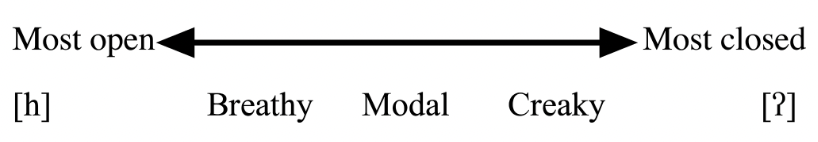
\includegraphics[width=.6\textwidth]{../Phonation.png}
	\caption{Simplified one-deminsional model for phonation. Based on \citet{ladefogedPreliminariesLinguisticPhonetics1971,gordonPhonationTypesCrosslinguistic2001}}.
	\label{fig:Phonation}
\end{figure}
\vspace{-2ex}
\begin{itemize}
	\item In addition to this degree of openness, linguists have found that there are other acoustic measurements that correlate to different types of phonation. 
	\item Commonly, these acoustic measurements are spectral-tilt measurements. 
	\item Spectral-tilt measurements are when you take the relative amplitude of different harmonics and subtract them from each other. 
	\item \cite{fischer-jorgensenPhoneticAnalysisBreathy1968} showed that the difference between the amplitude of the first harmonic (H1) and second harmonic (H2) can account for the differences between breathy and modal vowels.
	\item Further research has continued to rely on H1-H2, both corrected and uncorrected, to distinguish different types of phonation \citep[e.g.,][]{huffmanMeasuresPhonationType1987,klattAnalysisSynthesisPerception1990}. 
	\item Further research into spectral-tilt measurements began looking at other measurements besides H1-H2. These include looking at H1 minus the amplitude of the fourth harmonic (H4) or the amplitude of the harmonic closest to the different formants (A\textit{n}). 
	\item From these studies several patterns have emerged (see \cite{garellekPhoneticsVoice2019} for an overview). 
	\begin{itemize}
		\item Breathy phonation typically has a higher spectral-tilt measurement when compared to modal phonation. 
		\item Creaky phonation typically has a lower spectral-tilt measurement than modals. 
	\end{itemize} 
\end{itemize}

\begin{figure}[!h]
	\centering
	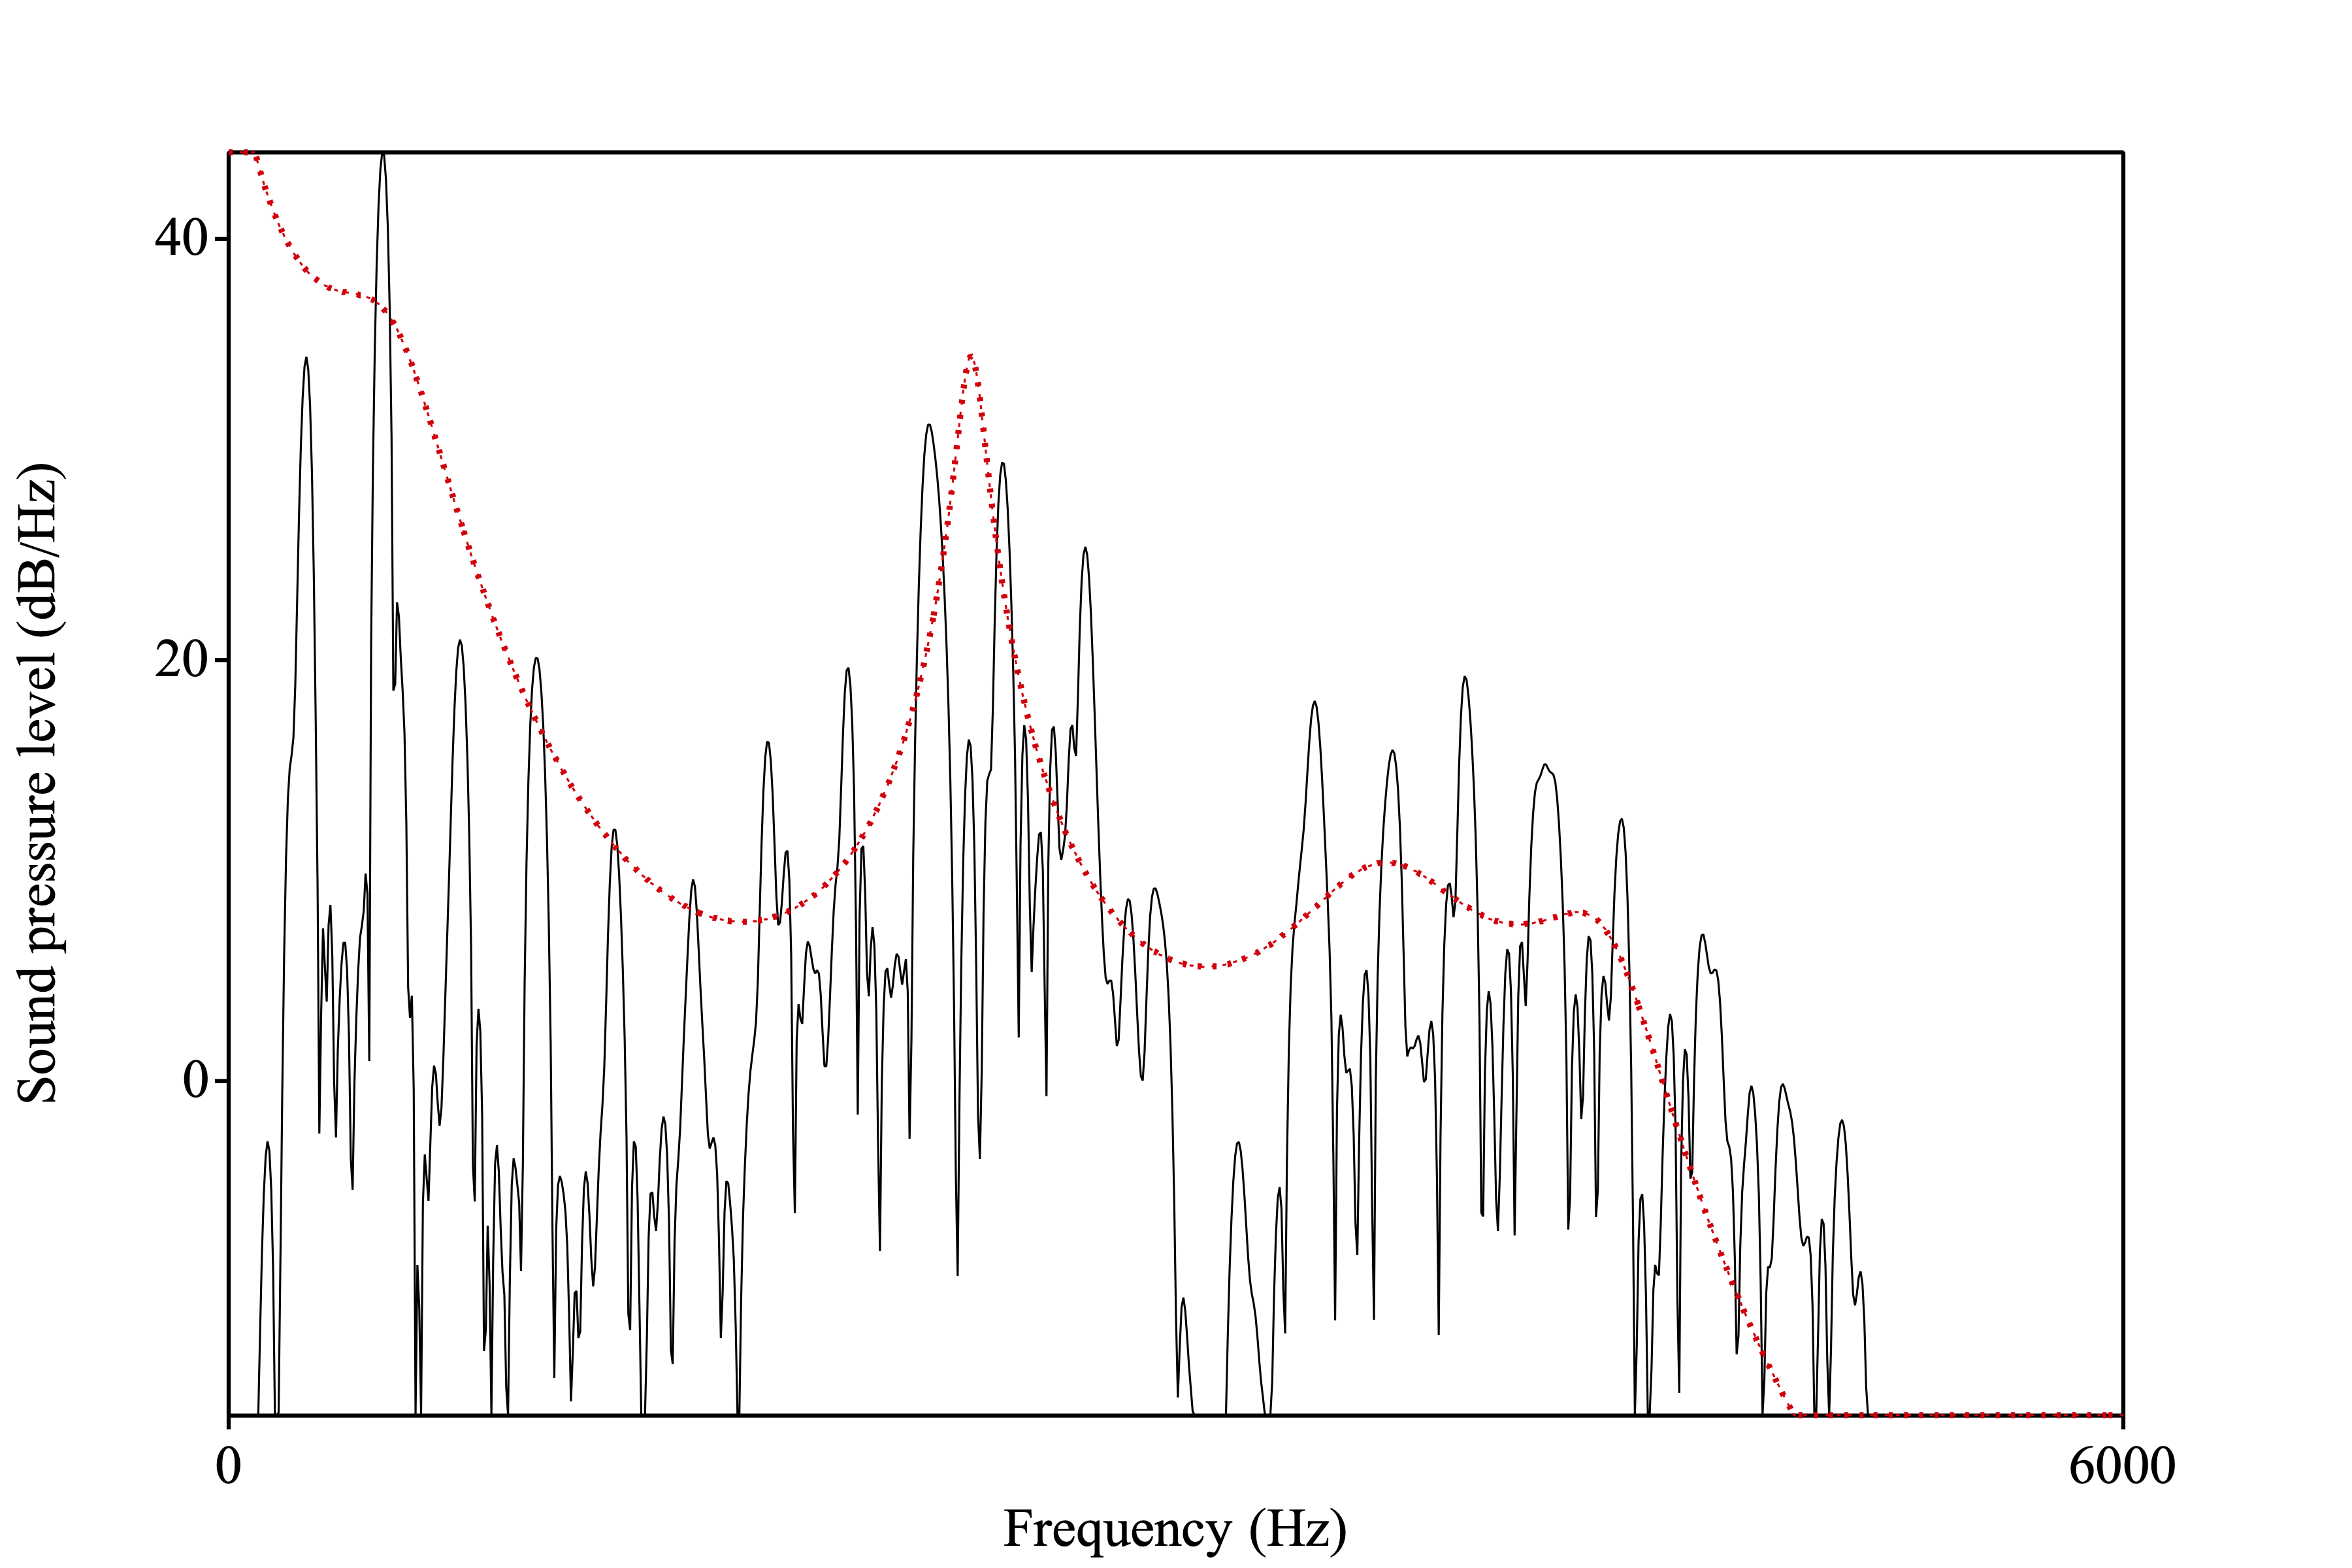
\includegraphics[width=0.9\textwidth]{../Harmonics.png}
	\caption{Spectral slice with LPC smoothed line overlaid for the vowel [e]. The harmonics in the spectral slice are represented by each of the dark peaks. The leftmost black solid line peak is the first harmonic (H1) and each subsequent peak represents the next highest harmonic (H2 through H\textit{n}). The red dotted line represents an LPC smoothed line which identifies the formants by the peaks in the line. Each of the harmonics that are closest to the formant peak is identified as A1 through A\textit{n}.}
	\label{fig:Harmonics}
\end{figure}
\vspace{-2ex}
\begin{itemize}
	\item The spectral-tilt measurement of H1-A3, the difference in amplitude between the first harmonic and the amplitude of the harmonic closest to the third formant, appears to be another of these measurements that robustly distinguishes different phonation types. 
	\item \citet{espositoVariationContrastivePhonation2010} found that in Central Valley Zapotecs, phonation contrasts were best captured by different measurements depending on sex. 
	\item H1-H2 was found to be effective only for female speakers, whereas male speakers were best characterized by H1-A3. 
	\item This pilot study will focus on these two spectral-tilt measurements.
	\item In addition to spectral-tilt measurements, measurements of noise frequently accompany investigations into phonation (e.g., \cite{garellekPhoneticsWhiteHmong2021}).
	\item One of the most commonly used measurements is Cepstral Peak Prominence (CPP; \cite{hillenbrandAcousticCorrelatesBreathy1994,hillenbrandAcousticCorrelatesBreathy1996}). 
	\item CPP is similar to the harmonics-to-noise ratio measure of \citet{dekromCepstrumBasedTechniqueDetermining1993} but differs in how the ‘prominence’ of the cepstral peak is calculated. 
	\item Prominence is taken as the difference in amplitude of the cepstral peak and a regression line used to normalize for window size and overall energy.
	\item A more prominent cepstral peak indicates stronger harmonics above the floor of the spectrum (i.e., greater periodicity in the speech signal).
	\item CPP was originally used as a diagnostic for breathy or modal voice \citep{blankenshipTimingNonmodalPhonation2002,espositoVariationContrastivePhonation2010} In fact, \citeauthor{espositoEffectsLinguisticExperience2010} showed that CPP was the best of the eight measures she considered for distinguishing modal from breathy phonation types.
	\item Further research has shown that CPP is also a good measurement for any type of non-modal phonation (e.g., \cite{andruskiPhonationTypesProduction2000,andruskiToneClarityMixed2006,blankenshipTimingNonmodalPhonation2002,waylandAcousticCorrelatesBreathy2003,avelinoAcousticElectroglottographicAnalyses2010}). 
	\item This will be the third measurement considered for this pilot study. 
\end{itemize}
%------------------------------------
\section{Santiago Laxopa Zapotec} \label{sec:SLZ}
%------------------------------------

\begin{itemize}
    \item Santiago Laxopa Zapotec (SLZ), endonym \textit{Dille'xhunh Laxup}, is a a Northern Zapotec language spoken by approximately 1000 people in the municipality of Santiago Laxopa, Ixtlán, Oaxaca, Mexico and in diaspora communities in Mexico and the United States \citep{adlerAcousticsPhonationTypes2016,adlerDerivationVerbInitiality2018,foleyForbiddenCliticClusters2018,foleyExtendingPersonCaseConstraint2020}.
    \item Closely related to San Bartolomé Zoogocho Zapotec \citep{longDiccionarioZapotecoSan2005,sonnenscheinDescriptiveGrammarSan2005} and shares a high level of mutual intelligibility with it.
    \item SLZ is similar to other Zapotecan languages in distinguishing lenis and fortis consonants \citep[e.g.,][]{nellisFortisLenisCajonos1980,jaegerFortisLenisQuestion1983,uchiharaFortisLenisGlides2016}.
\end{itemize}

\begin{table}[!h]
	\centering
	\caption{Consonant inventory for Santiago Laxopa Zapotec}
	\label{tab:SLZcons}
	\fittable{
	\begin{tabular}{llcccccccc}
	\lsptoprule
		  &  & bilabial & alveolar  & post- & retroflex & palatal &velar &labio-  &  uvular \\
		 &&&&alveolar&  &&&velar& \\
	\midrule
	stop 		& lenis   & b  & d  & & & & g & gʷ & \\
				& fortis  & p  & t  & & & & k & kʷ & \\
	fricative   & lenis   &    & z  & ʒ & ʐ &  & &  & ʁ \\
		        & fortis  &    & s  & ʃ & ʂ & ç & & & \\
	affricate 	& lenis   &    & d͡z & & & & & & \\
				& fortis  &    & t͡s & & t͡ʃ & & & & \\
    nasal    	& lenis   &	   & n  & & & & & & \\
				& fortis  &	mː & nː & & & & & & \\
	lateral  	& lenis   &    & l & & & & & & \\
				& fortis  &    & lː & & & & & & \\
	trill		& 		  &    & r & & &  & &  & \\ 			
	approximate & 		  &    & & & & & & w & \\ 
	\lspbottomrule
	\end{tabular}
	}
\end{table}

\begin{itemize}
    \item SLZ has a standard five vowel inventory. 
\end{itemize}

\begin{table}[!h]
	\centering
	\caption{Vowel qualities in Santiago Laxopa Zapotec.}
    \label{tab:SLZvowels}
	\begin{tabular}{lccc}
	\lsptoprule
	&  front& central  & back \\
	\midrule
	high   	&  i  &     &   u \\
	mid    	&  e  &   	& 	o \\
	low   	&     &  a 	&	  \\
	\lspbottomrule
	\end{tabular}
\end{table}

\begin{itemize}
	\item These five vowels, additionally, appear with one of four different phonation types which will be discussed in greater detail in Section~\ref{sec:Phonation}.
\end{itemize}

%------------------------------------
\subsection{Tone in Santiago Laxopa Zapotec} \label{sec:Tone}
%------------------------------------

\begin{itemize}
    \item Similar to other Otomanguean languages, SLZ is tonal \citep{suarezMesoamericanIndianLanguages1983,campbellMesoAmericaLinguisticArea1986,silvermanLaryngealComplexityOtomanguean1997,campbellOtomangueanHistoricalLinguistics2017a,campbellOtomangueanHistoricalLinguistics2017}.
    \item SLZ has five distinct tonal patterns that appear on the syllables of nouns, see Table~\ref{tab:tones}. 
\end{itemize}

\begin{table}[!h]
	\centering
	\caption{Examples of the five tonal patterns observed in the Santiago Laxopa Zapotec words.}
	\label{tab:tones}
	\begin{tabular}{lllll}
	\lsptoprule
	High   	&  a\supr{H}  &  \textit{xha}   &  [ ʐa\supr{H} ] & `clothing.\textsc{poss}'\\
	Mid    	&  a\supr{M}  &  \textit{lhill} 	& [ liʒ\supr{M} ] & `house.\textsc{poss}' \\
	Low   	&  a\supr{L}  &  \textit{yu'} 	&	 [ çuˀ\supr{L} ] & `earth'\\
	Rising	&  a\supr{MH}  &  \textit{yu'u} 	&	[ çuˀu\supr{MH} ] & `quicklime (Sp. cal)' \\
	Falling &  a\supr{HL}  &  \textit{yu'u}  &	[ çuˀu\supr{HL} ] &	`house' \\
	\lspbottomrule
	\end{tabular}
\end{table}

\begin{itemize}
	\item Figure~\ref{fig:FSRTonePlot} shows the five tonal contrasts averaged for each tonal contrast from the onset to ending of the vowel. 
	\item The first 20-25\% of Figure~\ref{fig:FSRTonePlot} can be ignored due to the influence of consonantal transitions. 
\end{itemize}

\begin{figure}[!ht]
	\centering
	\includegraphics[width=0.9\textwidth]{../FSRTonePlot.png}
	\caption{Tonal contrasts for FSR averaged and time normalized. Each line in this graph represents the average of approximately 10 syllables for each tonal pattern. }
	\label{fig:FSRTonePlot}
\end{figure}
%------------------------------------
\subsection{Phonation in Santiago Laxopa Zapotec} \label{sec:Phonation}
%------------------------------------

\begin{itemize}
	\item Zapotecan languages commonly make use of contrastive phonation on vowels \citep[e.g.,][]{avelinobecerraTopicsYalalagZapotec2004,avelinoAcousticElectroglottographicAnalyses2010,longDiccionarioZapotecoSan2005,lopeznicolasEstudiosFonologiaGramatica2016,chavez-peonInteractionMetricalStructure2010,ariza-garciaPhonationTypesTones2018}.
	\item SLZ has four contrastive phonation types, see (\ref{ex:YA})
\end{itemize}

\ea \label{ex:YA} Four-way near minimal phonation contrast
	\ea \textit{yag}  [çag\supr{L}] `tree; wood; almúd (unit of measurement approximately 4kg)'
	\ex \textit{yah}  [ça̤\supr{L}] `metal; rifle; bell'
	\ex \textit{yu'}  [çuˀ\supr{L}]  `earth'
	\ex \textit{ya'a}  [çaˀa\supr{L}]  `market'
	\z 
\z 

\begin{itemize}
	\item Breathy phonation on vowels is characterized by a raspy quality throughout the whole vowel or a portion toward the end of the vowel, see Figure~\ref{fig:BreathyVowel}. 
\end{itemize}
\vspace{-4ex}
\begin{figure}[!h]
	\centering
	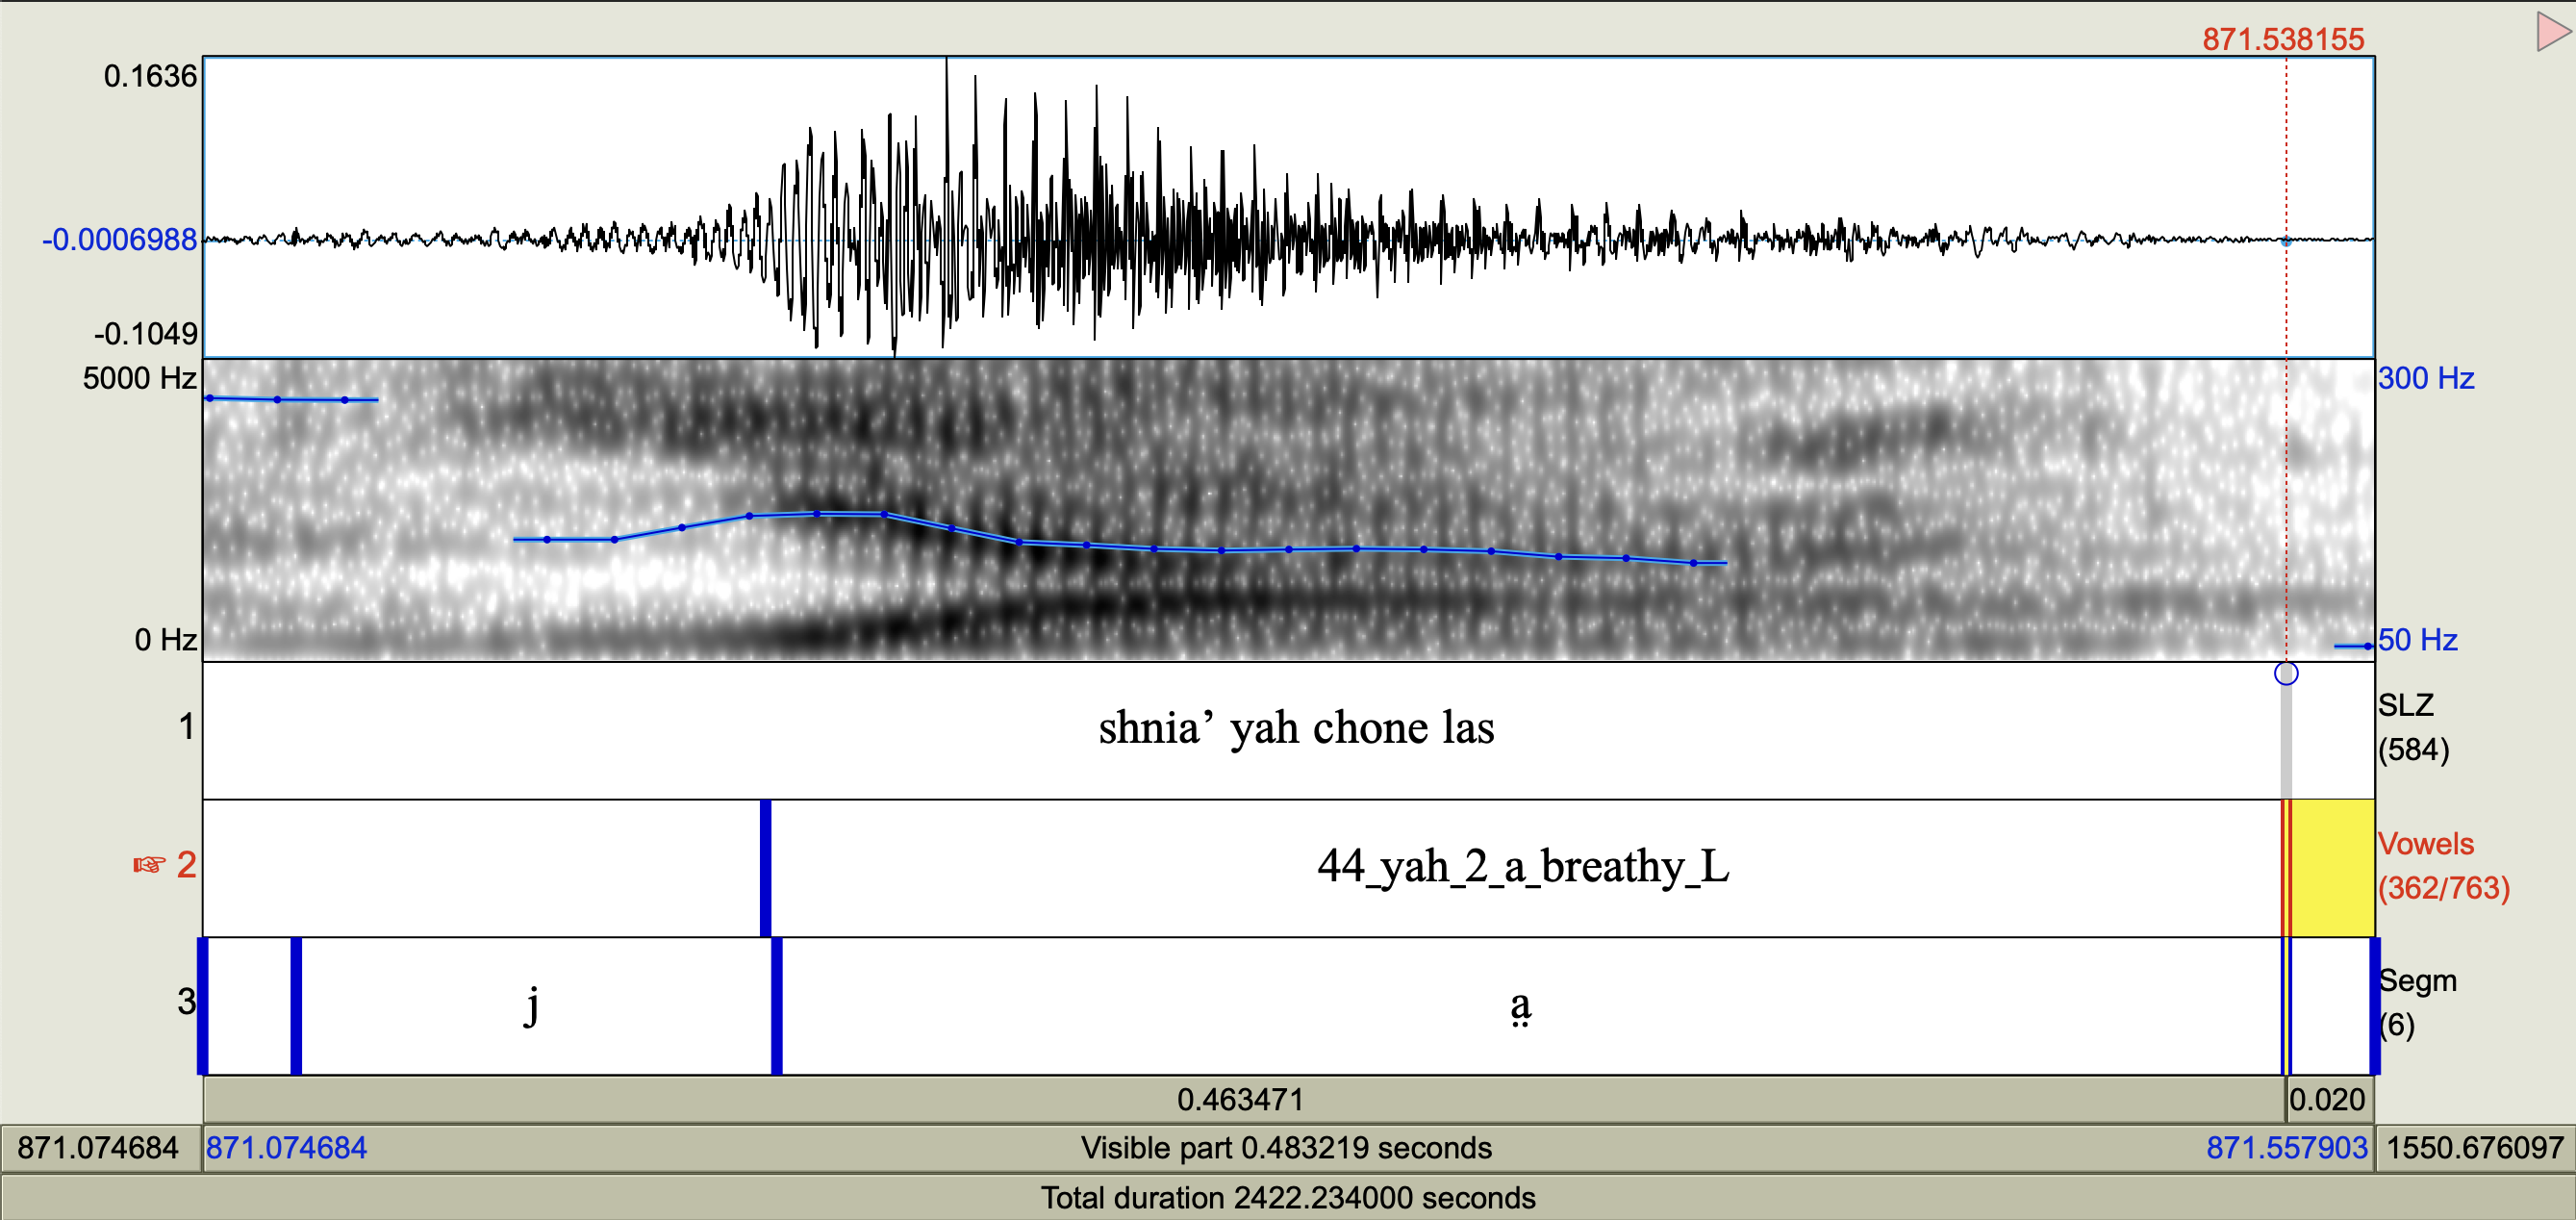
\includegraphics[width=0.9\textwidth]{../yah.png}
	\caption{FSR's breathy vowel in the word \textit{yah} `metal; rifle'}
	\label{fig:BreathyVowel}
\end{figure}

\begin{itemize}
	\item Checked vowels on the other hand are characterized by an abrupt glottal closure which cuts the vowel short. This phonation is sometimes only realized as a very short period of creakiness at the end of the vowel, see Figure~\ref{fig:CheckedVowel}.  
\end{itemize}
\vspace{-4ex}
\begin{figure}[!h]
	\centering
	% [INSERT YA SPECTROGRAM AND WAVEFORM]
	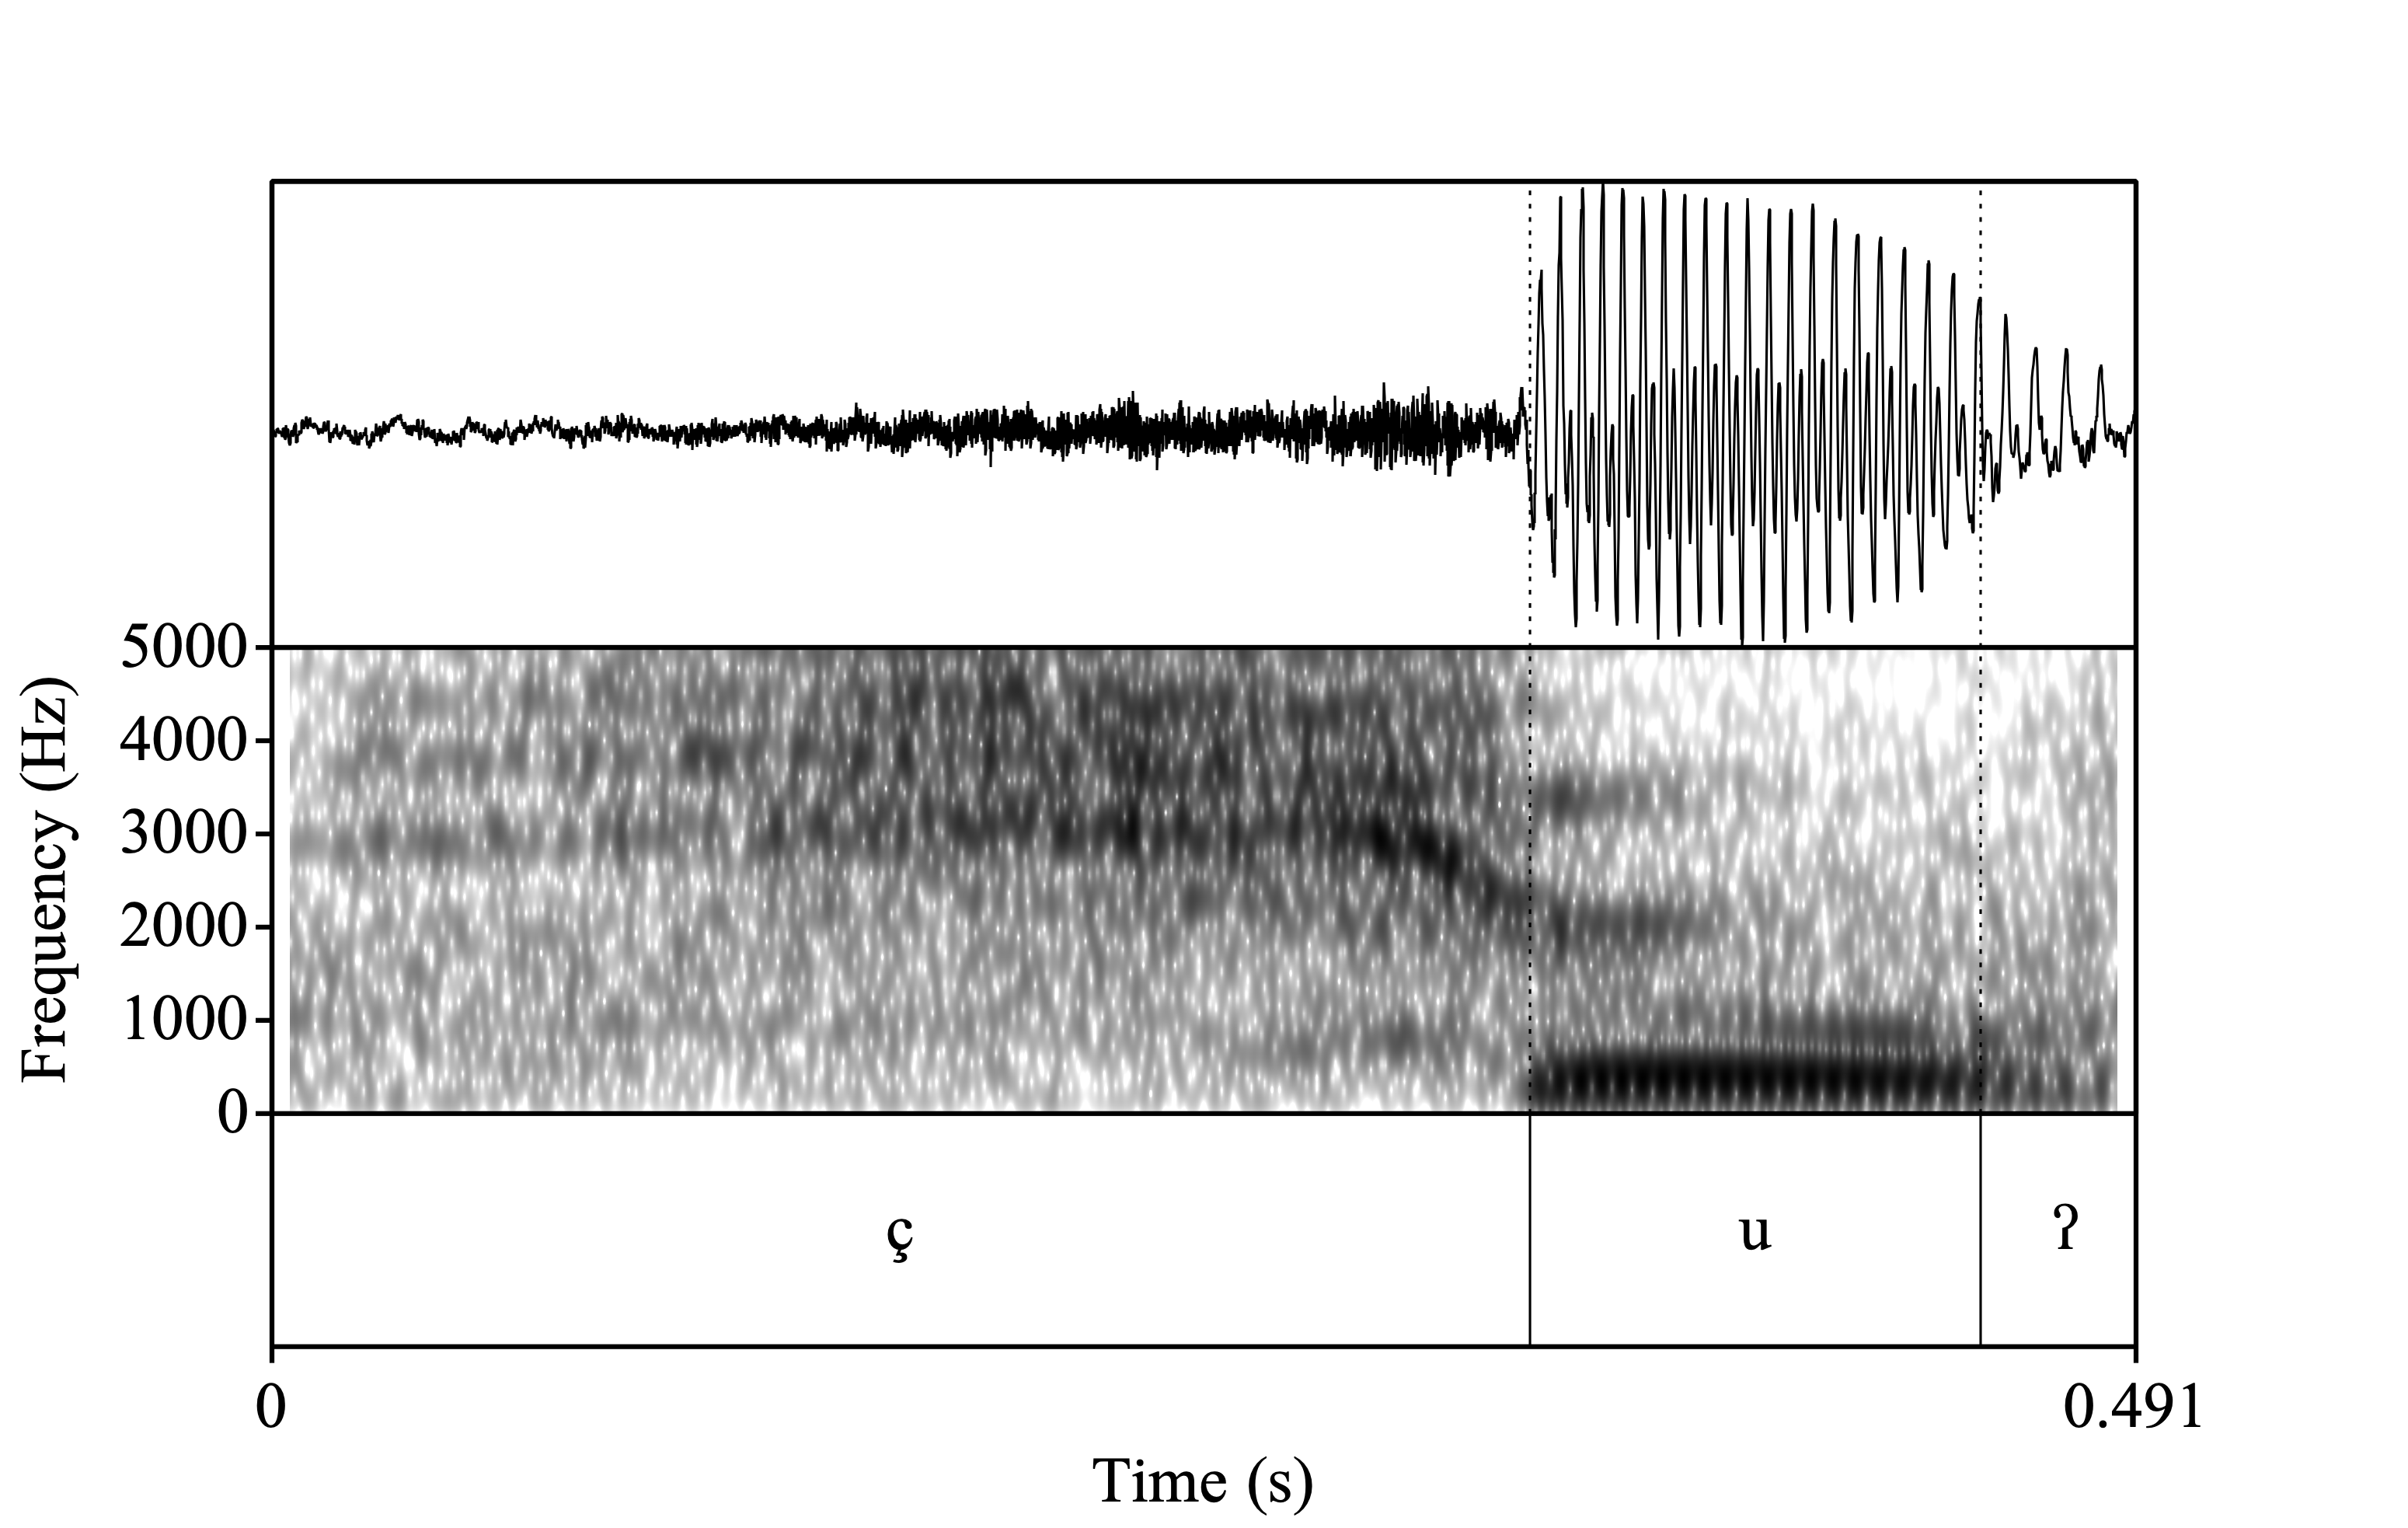
\includegraphics[width=0.9\textwidth]{../RD_yu'.png}
	\caption{RD's checked vowel in the word \textit{yu'} `earth'}
	\label{fig:CheckedVowel}
\end{figure}

\begin{itemize}
	\item Laryngealized vowels are quite common in Zapotecan languages and have received a wide number of different names. 
	\item Previous descriptions have used terms such as broken, rearticulated, interrupted, and creaky \citep{longDiccionarioZapotecoSan2005,avelinobecerraTopicsYalalagZapotec2004,avelinoAcousticElectroglottographicAnalyses2010,sonnenscheinDescriptiveGrammarSan2005,adlerAcousticsPhonationTypes2016,ariza-garciaPhonationTypesTones2018}.  
	\item In addition to a wide number of different names these vowels also exhibit a wide range of allophones.
	\item \citet{avelinoAcousticElectroglottographicAnalyses2010} found in the closely realted Yalálag Zapotec that among his consultants there were at least four different pronunciations as seen in Table~\ref{tab:laryngeal}. 
\end{itemize}

\begin{table}[!h]
	\centering
	\caption{Layngealized Vowels in Yalálag Zapotec}
	\label{tab:laryngeal}
	 \begin{tabular}{ll}
	\lsptoprule
	/VˀV/	&  [VʔV]  \\
			&  [VV̰V]   \\
			&  [VV̰ːV̆]  \\
			&  [VV̰V̰]	\\
	\lspbottomrule
	\end{tabular}
\end{table}

\begin{itemize}
	\item In SLZ, this vowel is also highly variable.
	\item One consultant does rearticulation, where there is a full glottal stop in the middle of the vowel, or creaky voice, see Figure~\ref{fig:FSRLaryngeal}. This alternation seems to be in free variation but there was a greater tendency to creak in words with a L tone, such as \textit{xa'ag} [ʂa̰ːx] `topil'\footnote{A topil is a type of government office in traditional Oaxacan communities somewhat akin to a sheriff.}.
	\item Another consultant only ever produced creaky voice for these vowels regardless of the tone with the word, see Figure~\ref{fig:RDLaryngeal}.
	\item Further research will show whether these differences are sociolinguistic in nature or whether these differences are individualistic. 
\end{itemize}

\begin{figure}[!h]
	\centering
	\begin{subfigure}{.5\textwidth}
		\centering
		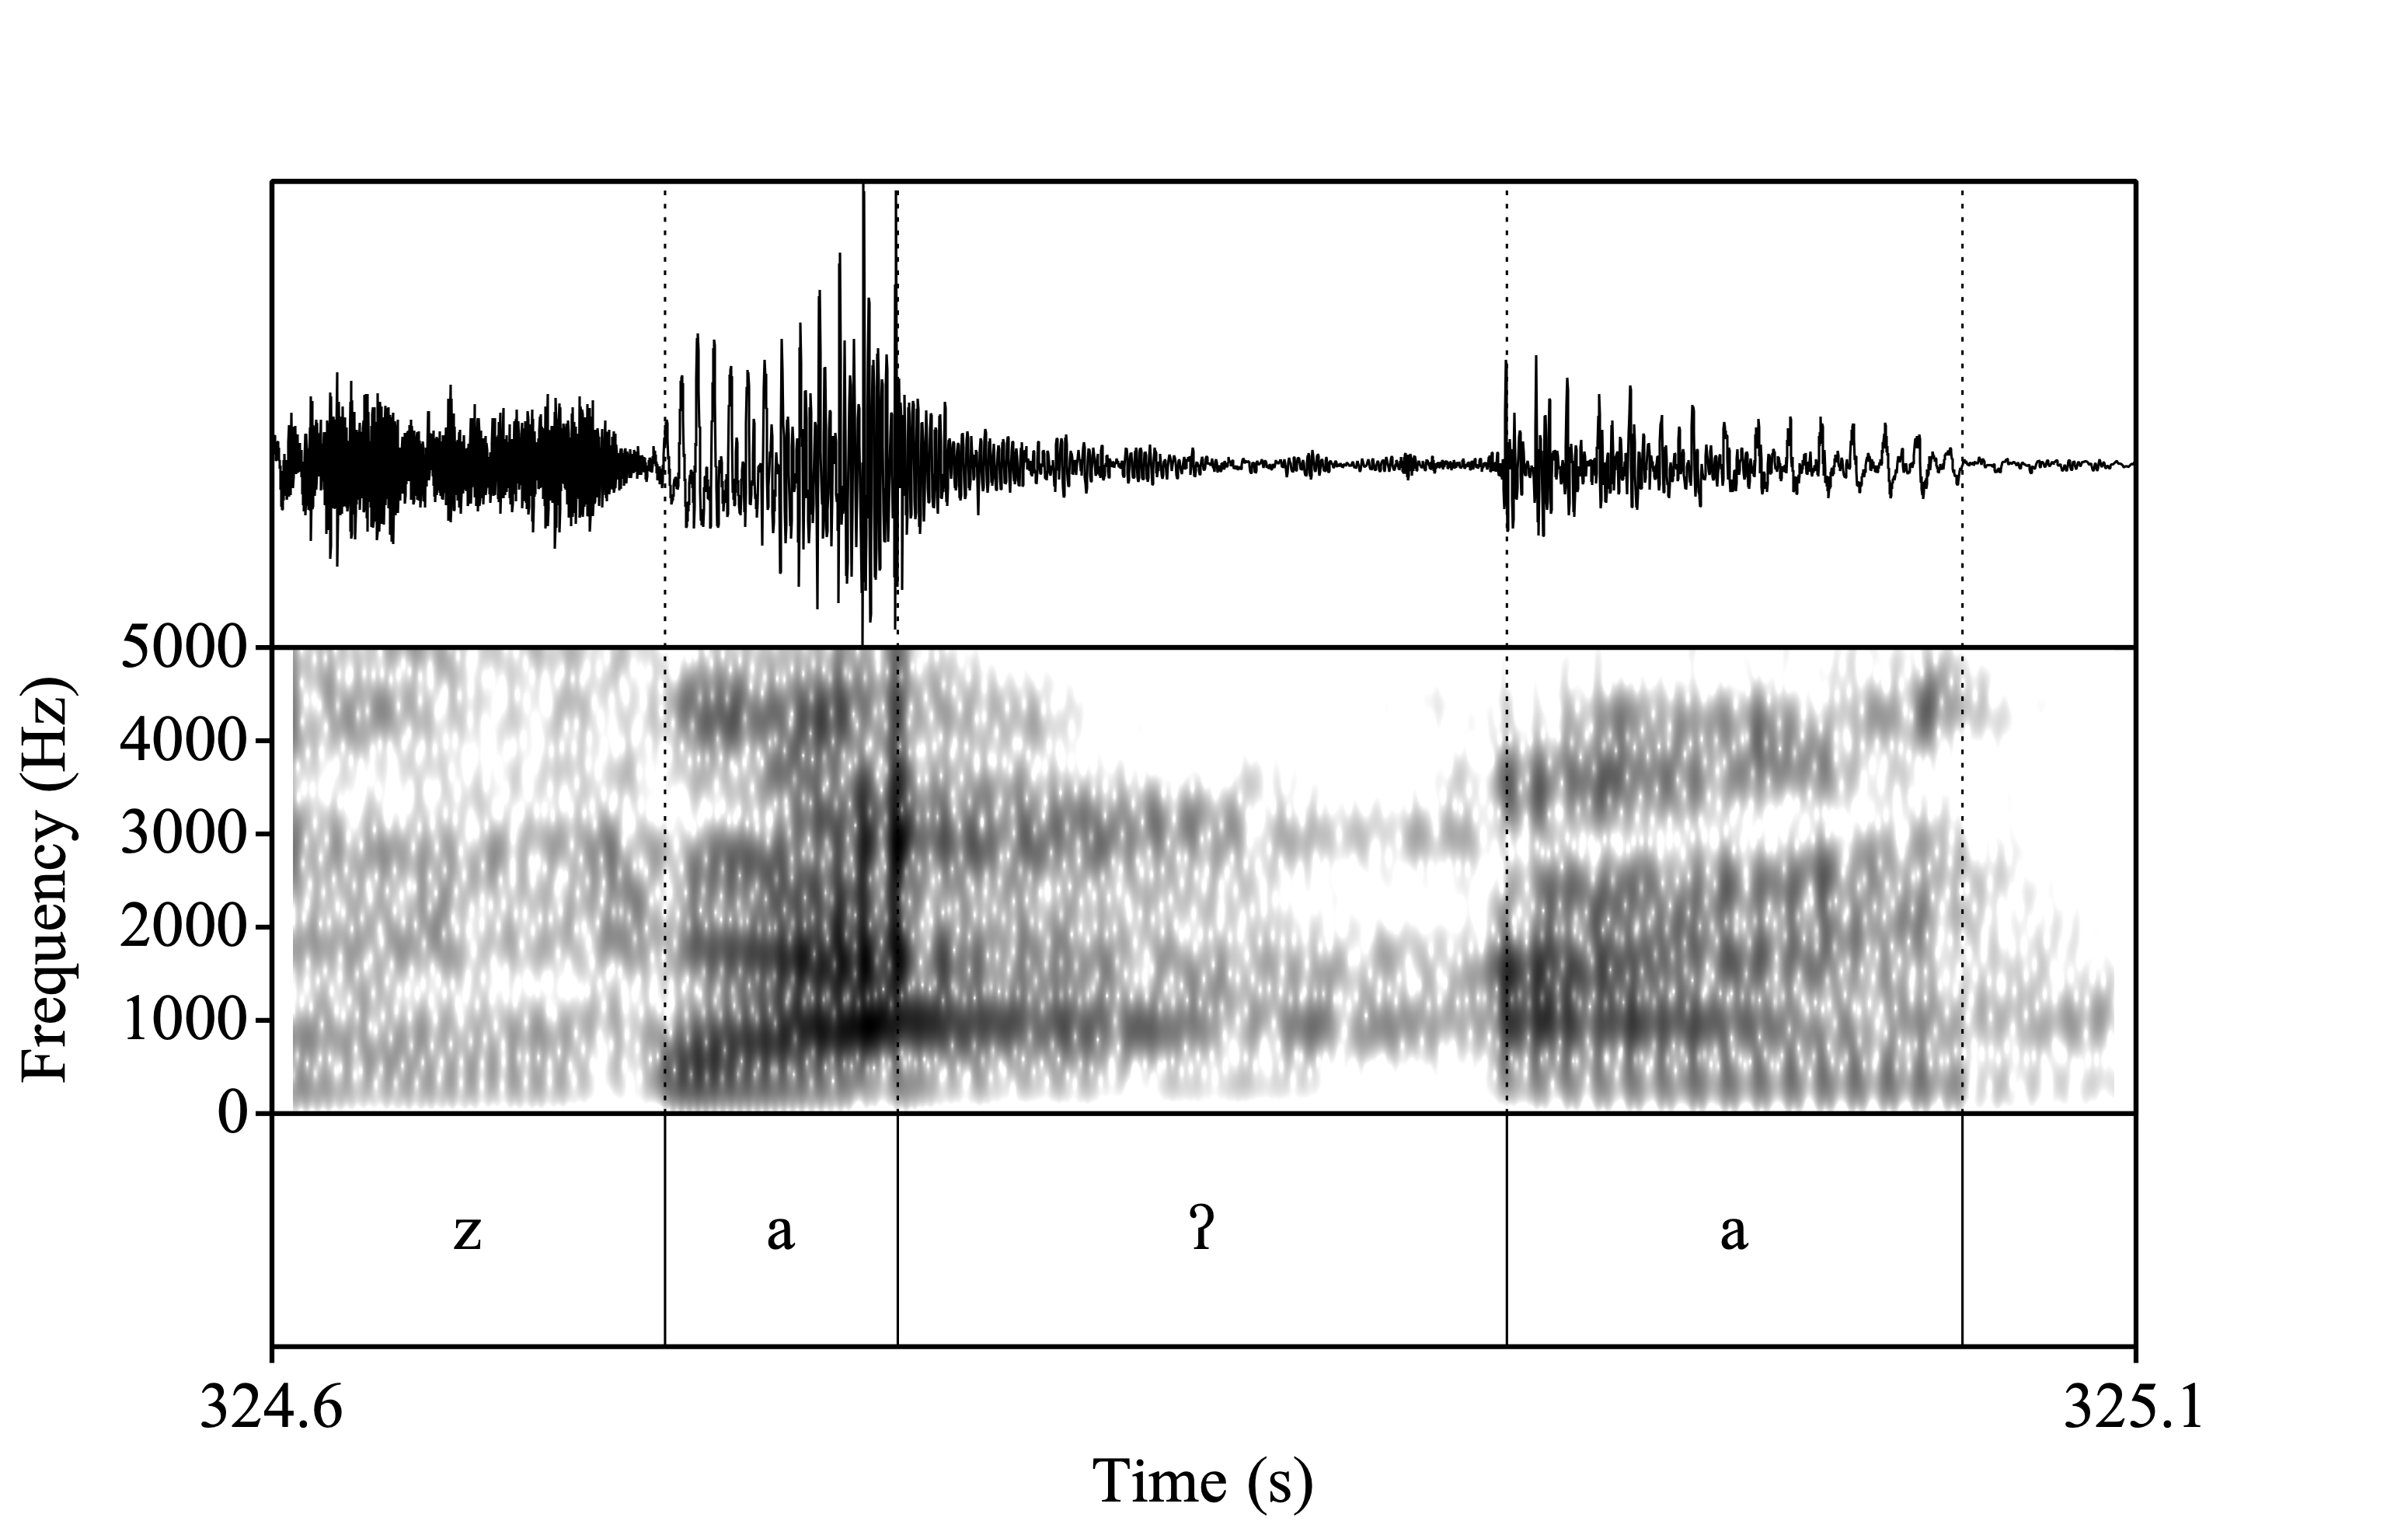
\includegraphics[width=\linewidth]{../za'a.png}
		\caption{\textit{za'a} `corncob'}
		\label{fig:za'a}
	\end{subfigure}%
	\begin{subfigure}{.5\textwidth}
		\centering
		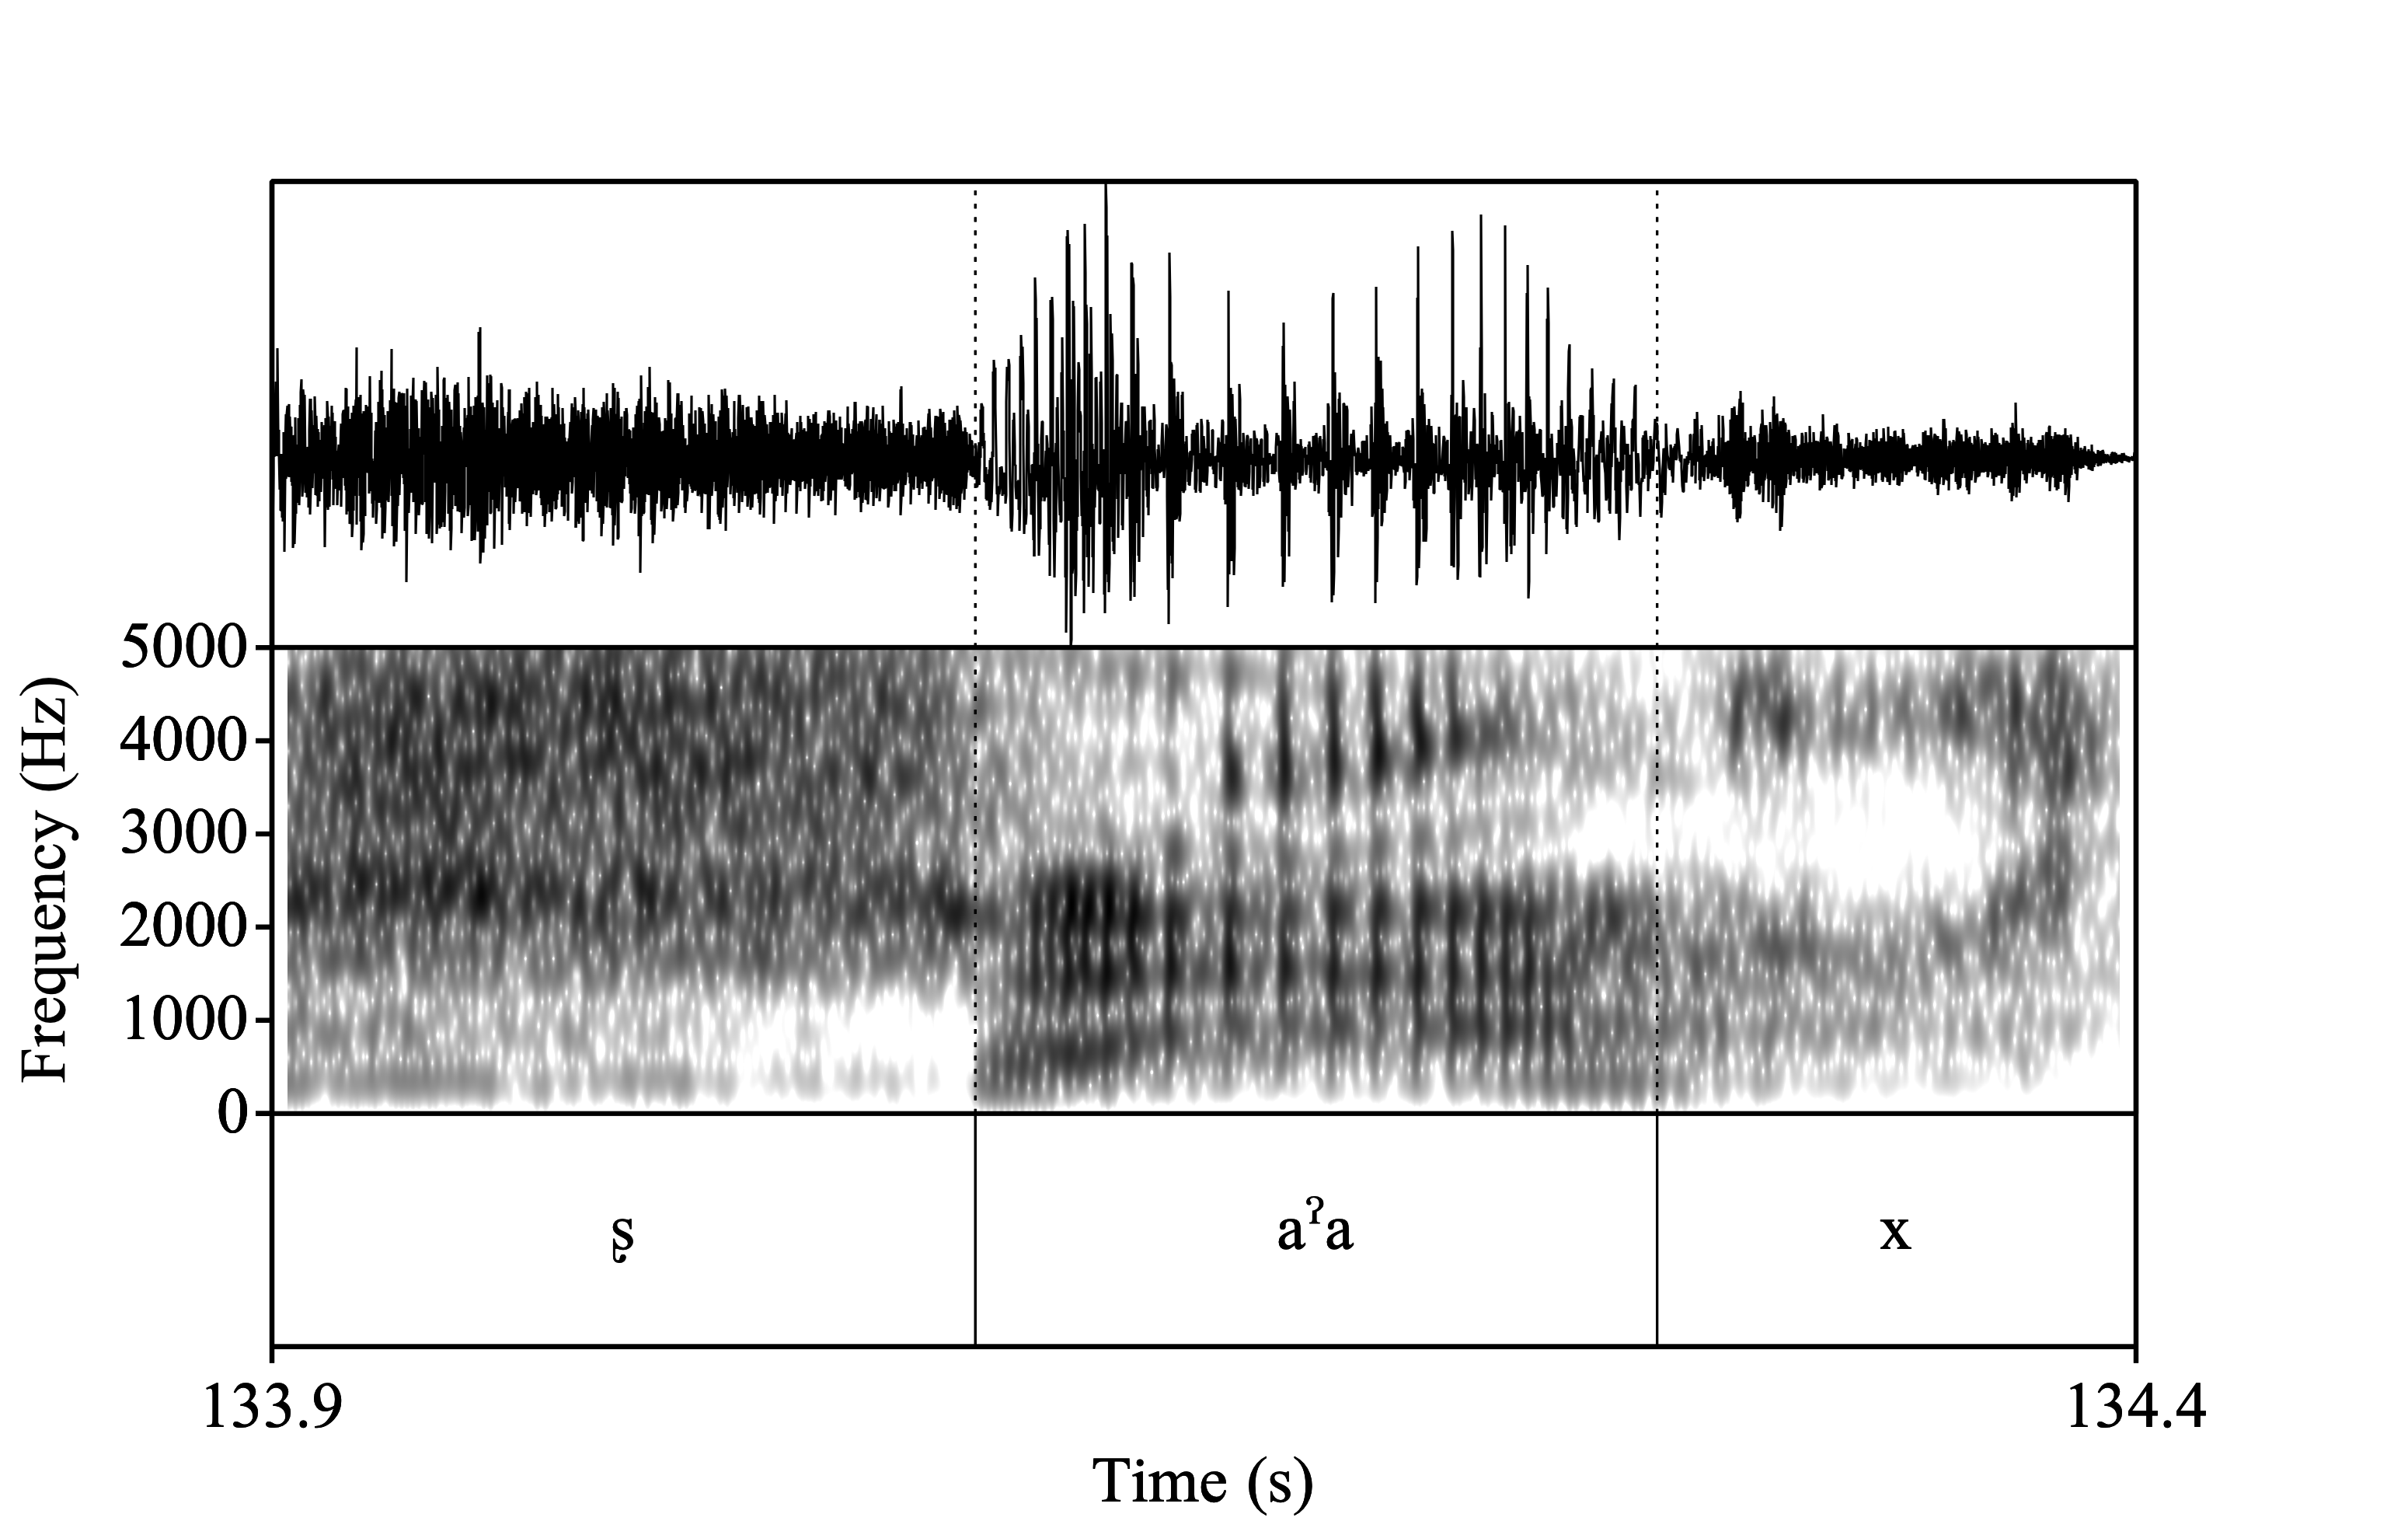
\includegraphics[width=\linewidth]{../xa'ag.png}
		\caption{\textit{xa'ag} `topil'}
		\label{fig:xa'ag}
	\end{subfigure}	
	\caption{Comparison of FSR's laryngealized vowels in \textit{za'a} `corncob' and \textit{xa'ag} `topil'}
	\label{fig:FSRLaryngeal}
\end{figure}

\begin{figure}[!h]
	\centering
	\begin{subfigure}{.5\textwidth}
		\centering
		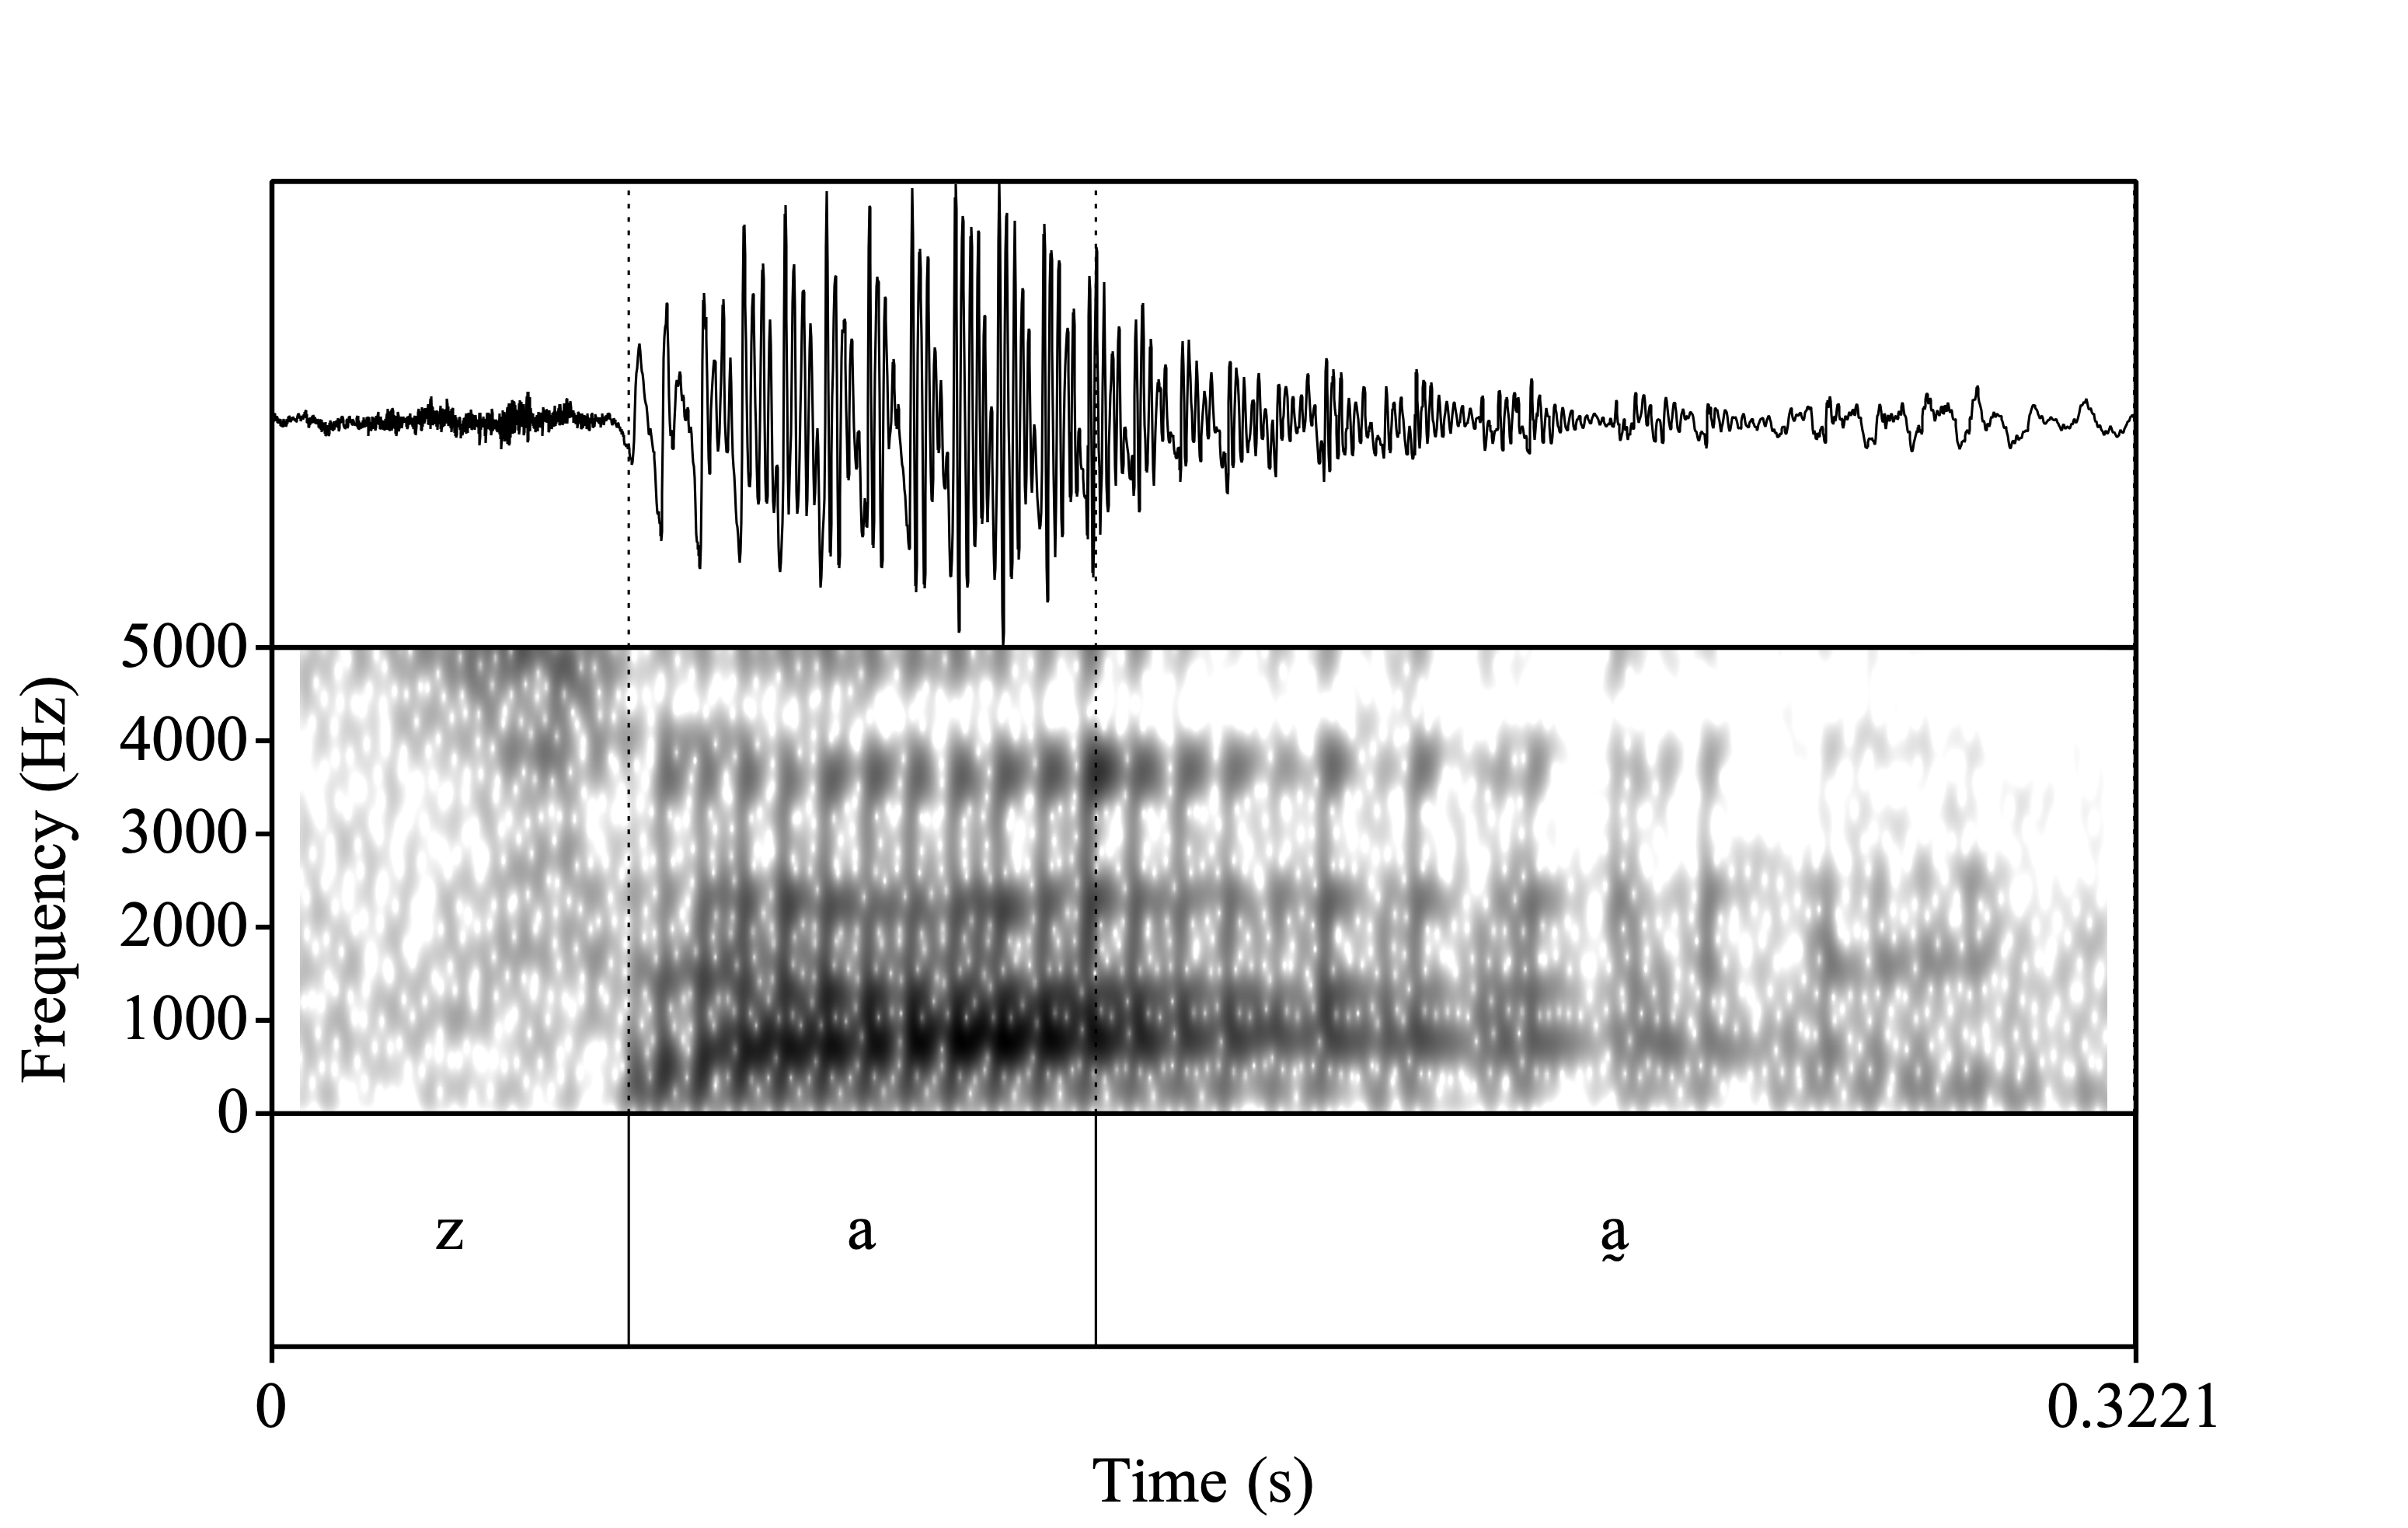
\includegraphics[width=\linewidth]{../RD_za'a.png}
		\caption{\textit{za'a} `corncob'}
		\label{fig:za'a}
	\end{subfigure}%
	\begin{subfigure}{.5\textwidth}
		\centering
		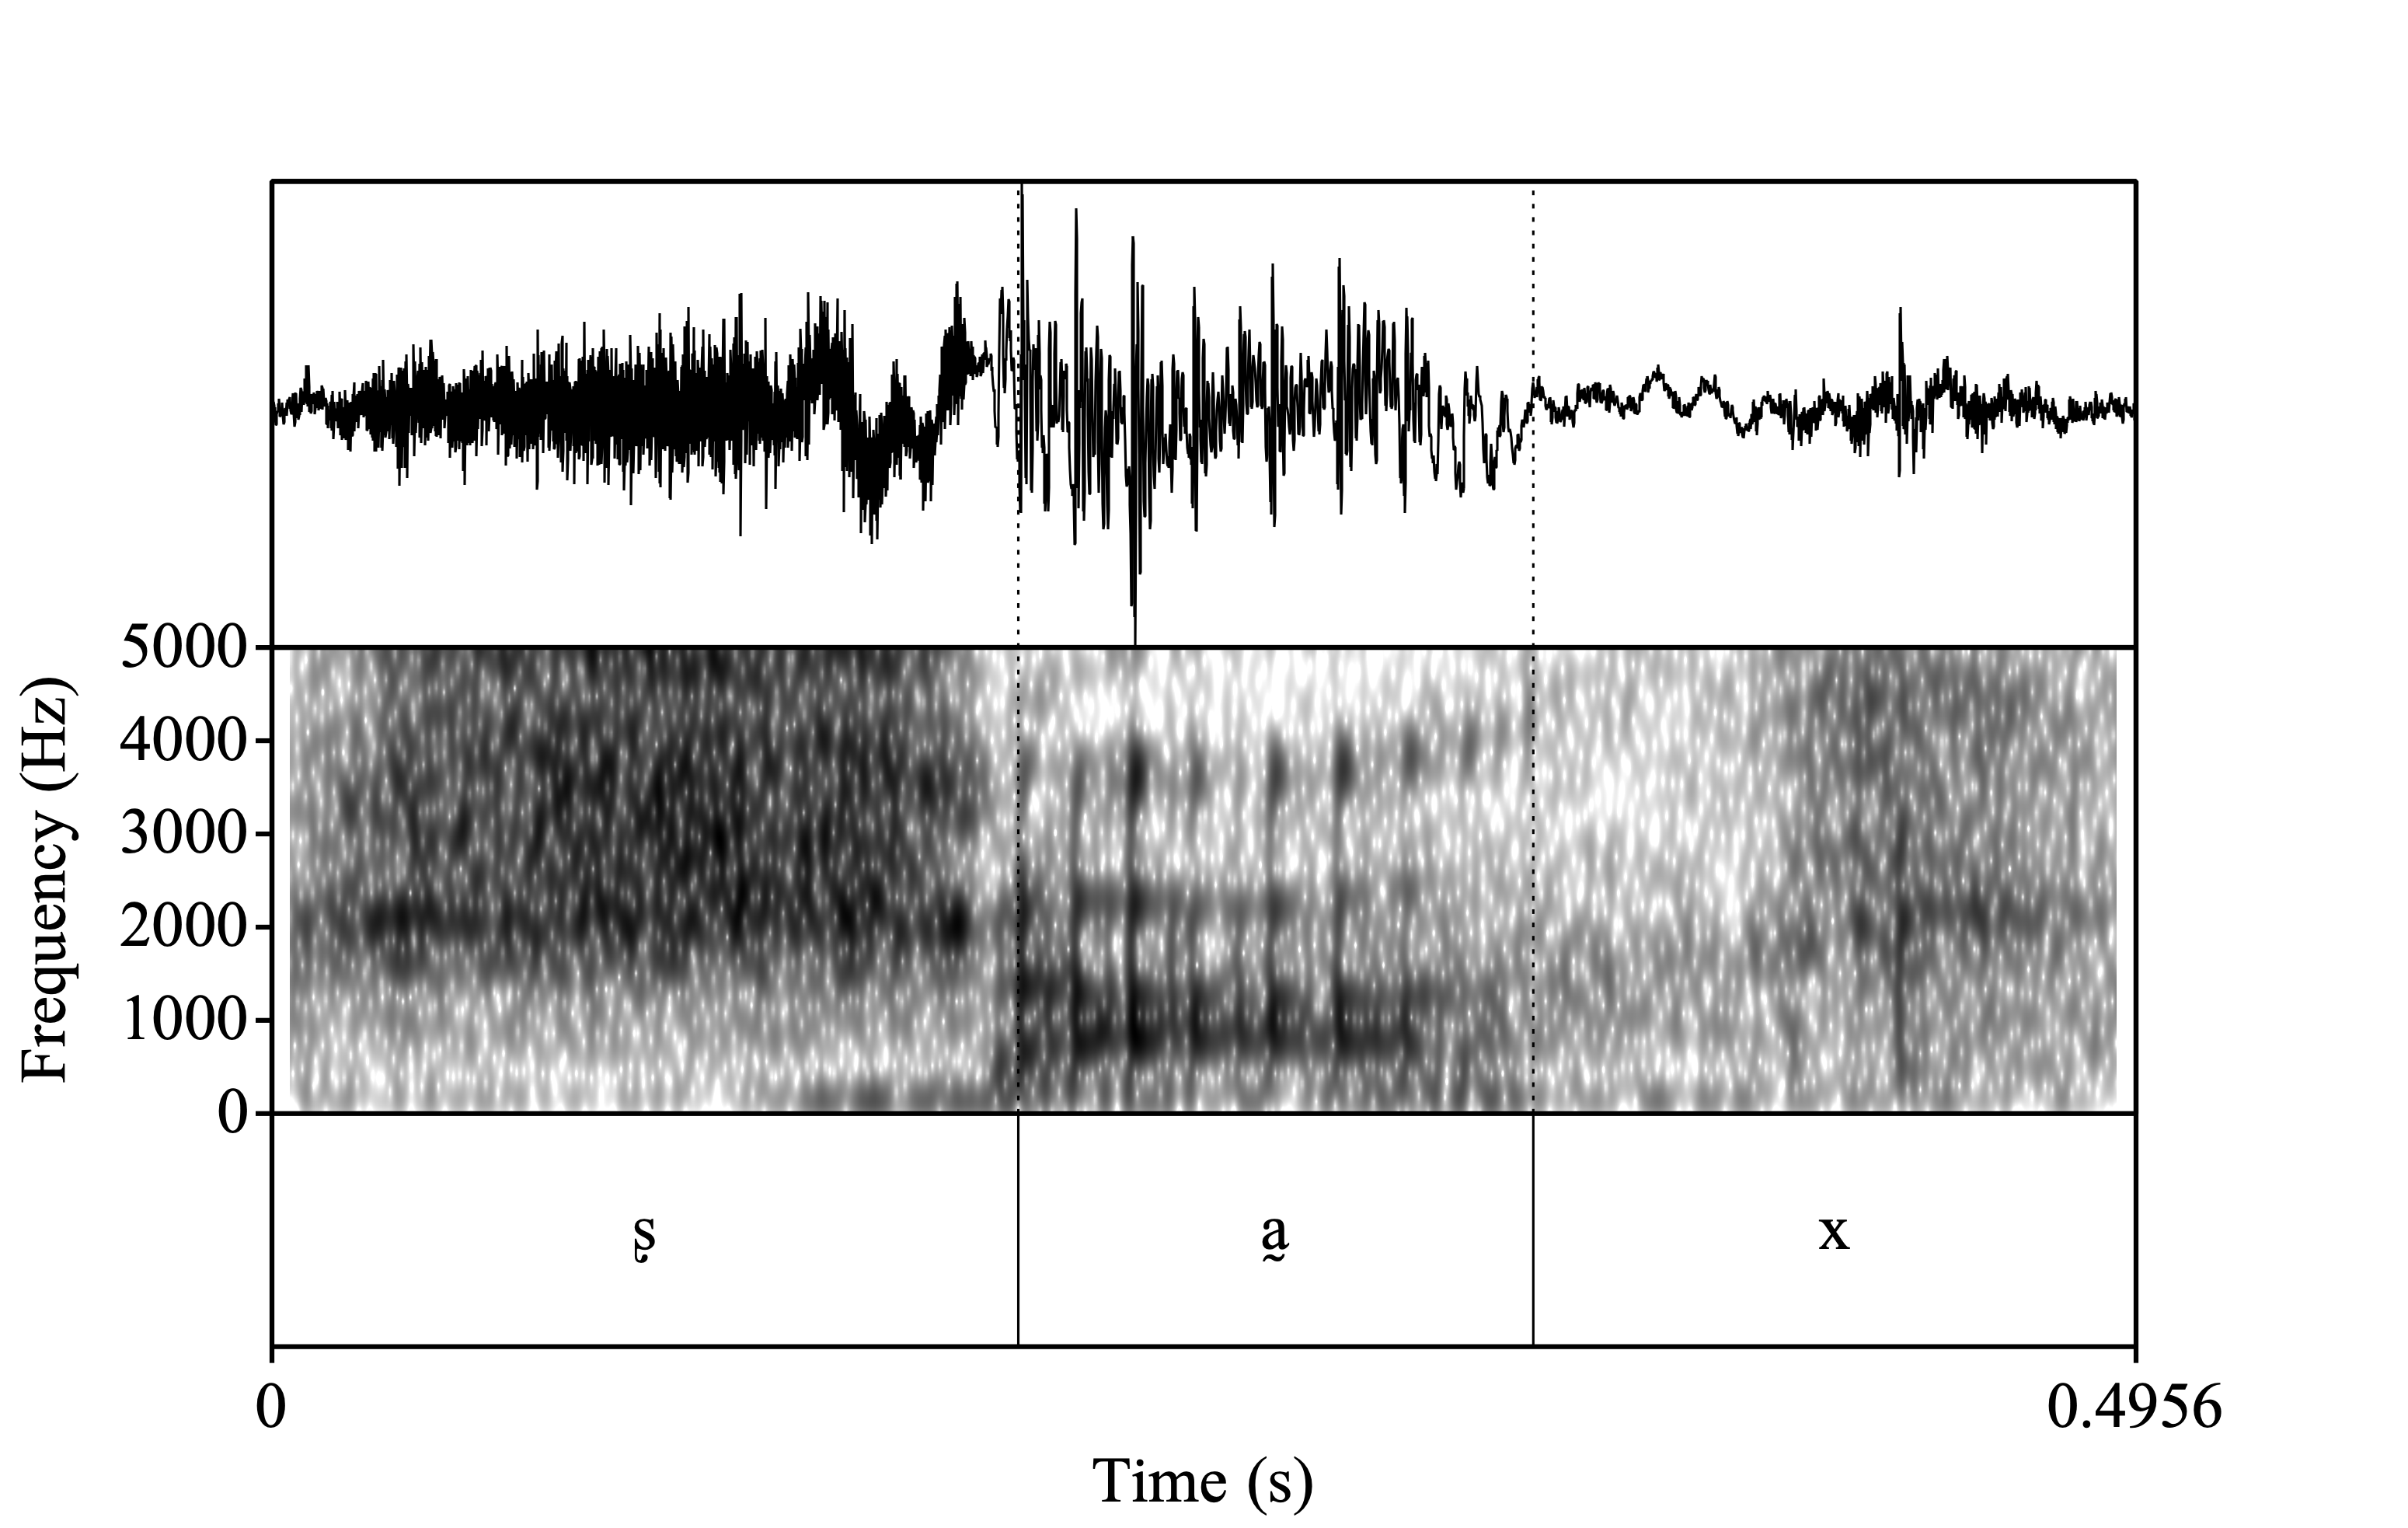
\includegraphics[width=\linewidth]{../RD_xa'ag.png}
		\caption{\textit{xa'ag} `topil'}
		\label{fig:xa'ag}
	\end{subfigure}
	\caption{Comparison of RD's laryngealized vowels in \textit{za'a} `corncob' and \textit{xa'ag} `topil'}
	\label{fig:RDLaryngeal}
\end{figure}

%------------------------------------
\subsection{Interaction of tone and phonation in Santiago Laxopa Zapotec} \label{sec:TonePhonation}
%------------------------------------

\begin{itemize}
	\item Most previous work on the interaction of tone has been focused on the languages of East and Southeast Asia 
	\citep[e.g.,][]{masicaDefiningLinguisticArea1976,thurgoodVietnameseTonogenesisRevising2002,yipTone2002,enfieldArealLinguisticsMainland2005,michaudComplexTonesEast2012,brunelleTonePhonationSoutheast2016}.
	\item \citet{smalleyProblemsConsonantsTone1976} and \citet{ratliffMeaningfulToneStudy1992} both describe White Hmong's (Hmong-Mien) \textit{-g} tone as being a mid-low tone with breathy phonation
	\item Mandarin's (Sino-Tibetan) tone 3 is often associated with creaky phonation \citep{hockettPeipingPhonology1947}. \citet{brunelleTonePerceptionNorthern2009} found that creaky phonation plays an important role in the production of certain tones. 
	\item Additionally, work on S'gaw Karen (Sino-Tibetan) has found that two tones are only differentiated by the presence of some form of non-modal phonation (Boehm p.c.). 
	\item In Oto-Manguean languages, there is strong evidence that tone and phonation are independent from each other \citep[e.g.,][]{silvermanLaryngealComplexityOtomanguean1997,avelinobecerraTopicsYalalagZapotec2004,avelinoAcousticElectroglottographicAnalyses2010, chavez-peonInteractionMetricalStructure2010, campbellZenzontepecChatinoAspect2011,garellekAcousticConsequencesPhonation2011,villardPhonologyMorphologyZacatepec2015, lopeznicolasEstudiosFonologiaGramatica2016,ariza-garciaPhonationTypesTones2018}. 
	\item In San Lucas Quiaviní Zapotec (Valley Zapotec) almost all of the the different tones and phonation types can be combined with each other.
	\item The rising tone in SLQZ is restricted to only appearing with modal voice. 
\end{itemize}

\begin{table}[!ht]
	\centering
	\caption{SLQZ tone and phonation interactions \citep{chavez-peonInteractionMetricalStructure2010}.}
	\label{tab:SLQZ}
	 \begin{tabular}{lcccc}
	  \lsptoprule
					  &	 \textbf{Modal}  & \textbf{Breathy} & \textbf{Creaky} & \textbf{Interrupted} \\
		  High	& ✔︎ & -- & ✔︎ & ✔︎ \\
		  Low & ✔︎ & ✔︎ & ✔︎ & ✔︎ \\
		  Falling & ✔︎ & ✔︎ & ✔︎ & ✔︎ \\
		  Rising & ✔︎ & -- & -- & -- \\
	  \lspbottomrule
	 \end{tabular}
\end{table}

\begin{itemize}
	\item SLZ is similar to SLQZ in allowing almost all combinations of tone and phonation. 
	\item There are two gaps in the distribution of tone and phonation: Breathy-High and Checked-Falling. 
\end{itemize}

\begin{table}[!h]
	\caption{Observed combinations of tone and phonation in SLZ.}
	\label{tab:ToneVoiceQuality}
	\centering

	\begin{tabular}{lcccc}
	\lsptoprule
		& \textbf{Modal} & \textbf{Breathy} & \textbf{Checked} & \textbf{Laryngealized} \\
	\hline
	High		& ✔︎ & -- & ✔︎ & ✔︎ \\
	Mid			& ✔︎ & ✔︎  & ✔︎ & ✔︎ \\
	Low			& ✔︎ & ✔︎  & ✔︎ & ✔︎ \\
	Rising		& ✔︎ & ✔︎  & ✔︎ & ✔︎ \\
	Falling		& ✔︎ & ✔︎  & --	& ✔︎ \\
	\lspbottomrule
	\end{tabular}
\end{table}

\begin{itemize}
	\item This gap of breathy phonation and high tone is quite common across the Zapotecan languages (Campbell p.c.). 
	\item In the case of breathy phonation in SLQZ, \citet{uchiharaToneRegistrogenesisQuiavini2016} offers some convincing evidence that the phonation originated in syllables with low tone and then spread to other tones via analogy.
\end{itemize}

%------------------------------------
\section{Methodology} \label{sec:Methods}
%------------------------------------

\begin{itemize}
	\item Two native language speakers of SLZ who live in Santa Cruz, CA took part in this study (one male). 
	\item Because of the COVID-19 pandemic data collection was conducted remotely using Zencastr, a professional podcasting website, (44.1kHz, 16-bit) or in-person outside in a well ventilated location, using a Zoom H4n handheld recorder (44.1kHz, 16-bit).
	\item The SLZ speakers were recorded saying approximately 100 words in isolation three times and those same words three times in the carrier phrase \textit{shnia' X chonhe lhas} `I say X three times'. 
	\item The resulting files were first segmented in ELAN \citep{wittenburgELANProfessionalFramework2006} then each individual vowel from the target word was isolated from the carrier sentences using Praat \citep{boersmaPraatDoingPhonetics2021}. 
	\item After isolating each vowel token the files were fed into VoiceSauce \citep{shueVOICESAUCEProgramVoice2009} for calculating the different spectral-tilt and noise measurements. 
	\item Each vowel was normalized for time and then the various acoustic measurements were averaged for each third of the vowel following \citet{garellekAcousticConsequencesPhonation2011}.
\end{itemize}

%------------------------------------
\section{Results} \label{sec:Results}
%------------------------------------

%------------------------------------
\subsection{H1-H2 spectral-tilt results} \label{sec:H1H2}
%------------------------------------

\begin{itemize}
	\item In all three portions of the vowels, H1-H2 was not a very good measure for spectral-tilt in this variety of Zapotec. 
	\item In all three thirds of the vowel, we see very little differences in the values for H1-H2 between modal, checked, and laryngealized.  
	\item In the first third of the vowel there are virtually no differences between the four phonation types, see Figure~\ref{fig:h1h2first}.
\end{itemize}

\begin{figure}[!ht]
	\centering
	\begin{subfigure}{.5\textwidth}
		\centering
		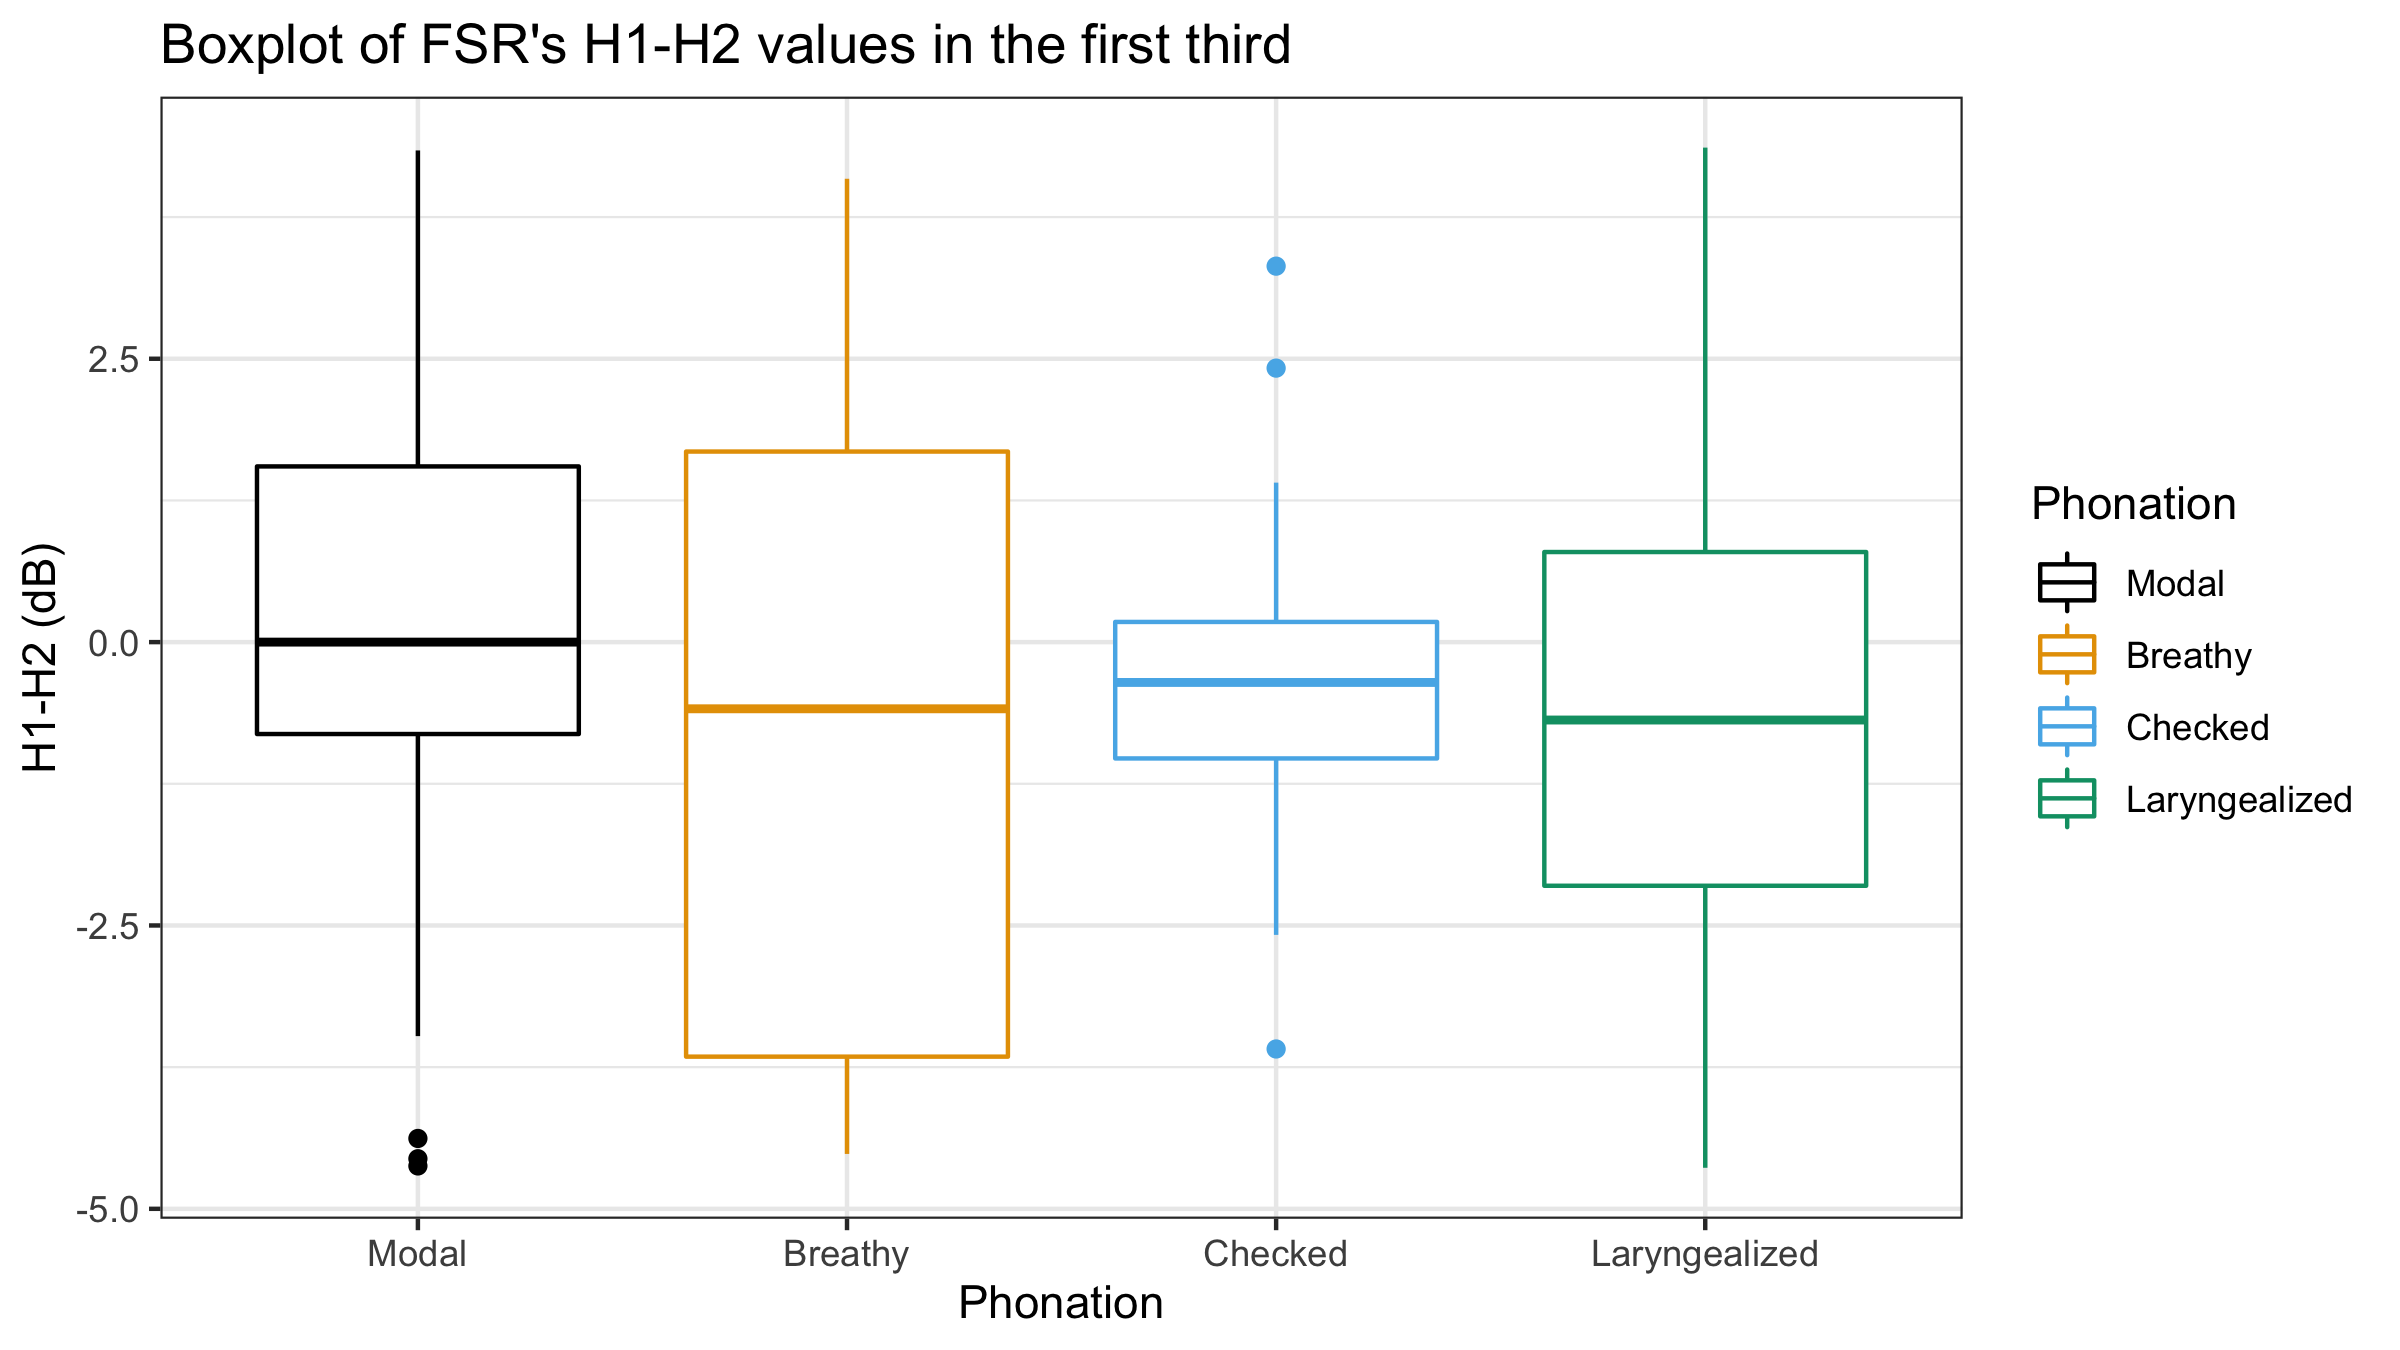
\includegraphics[width=0.9\textwidth]{../mean_FSR_h1h2_1st.png}
		\caption{FSR's H1-H2 values.}
		\label{fig:FSRh1h2first} 
	\end{subfigure}%
	\begin{subfigure}{.5\textwidth}
		\centering
		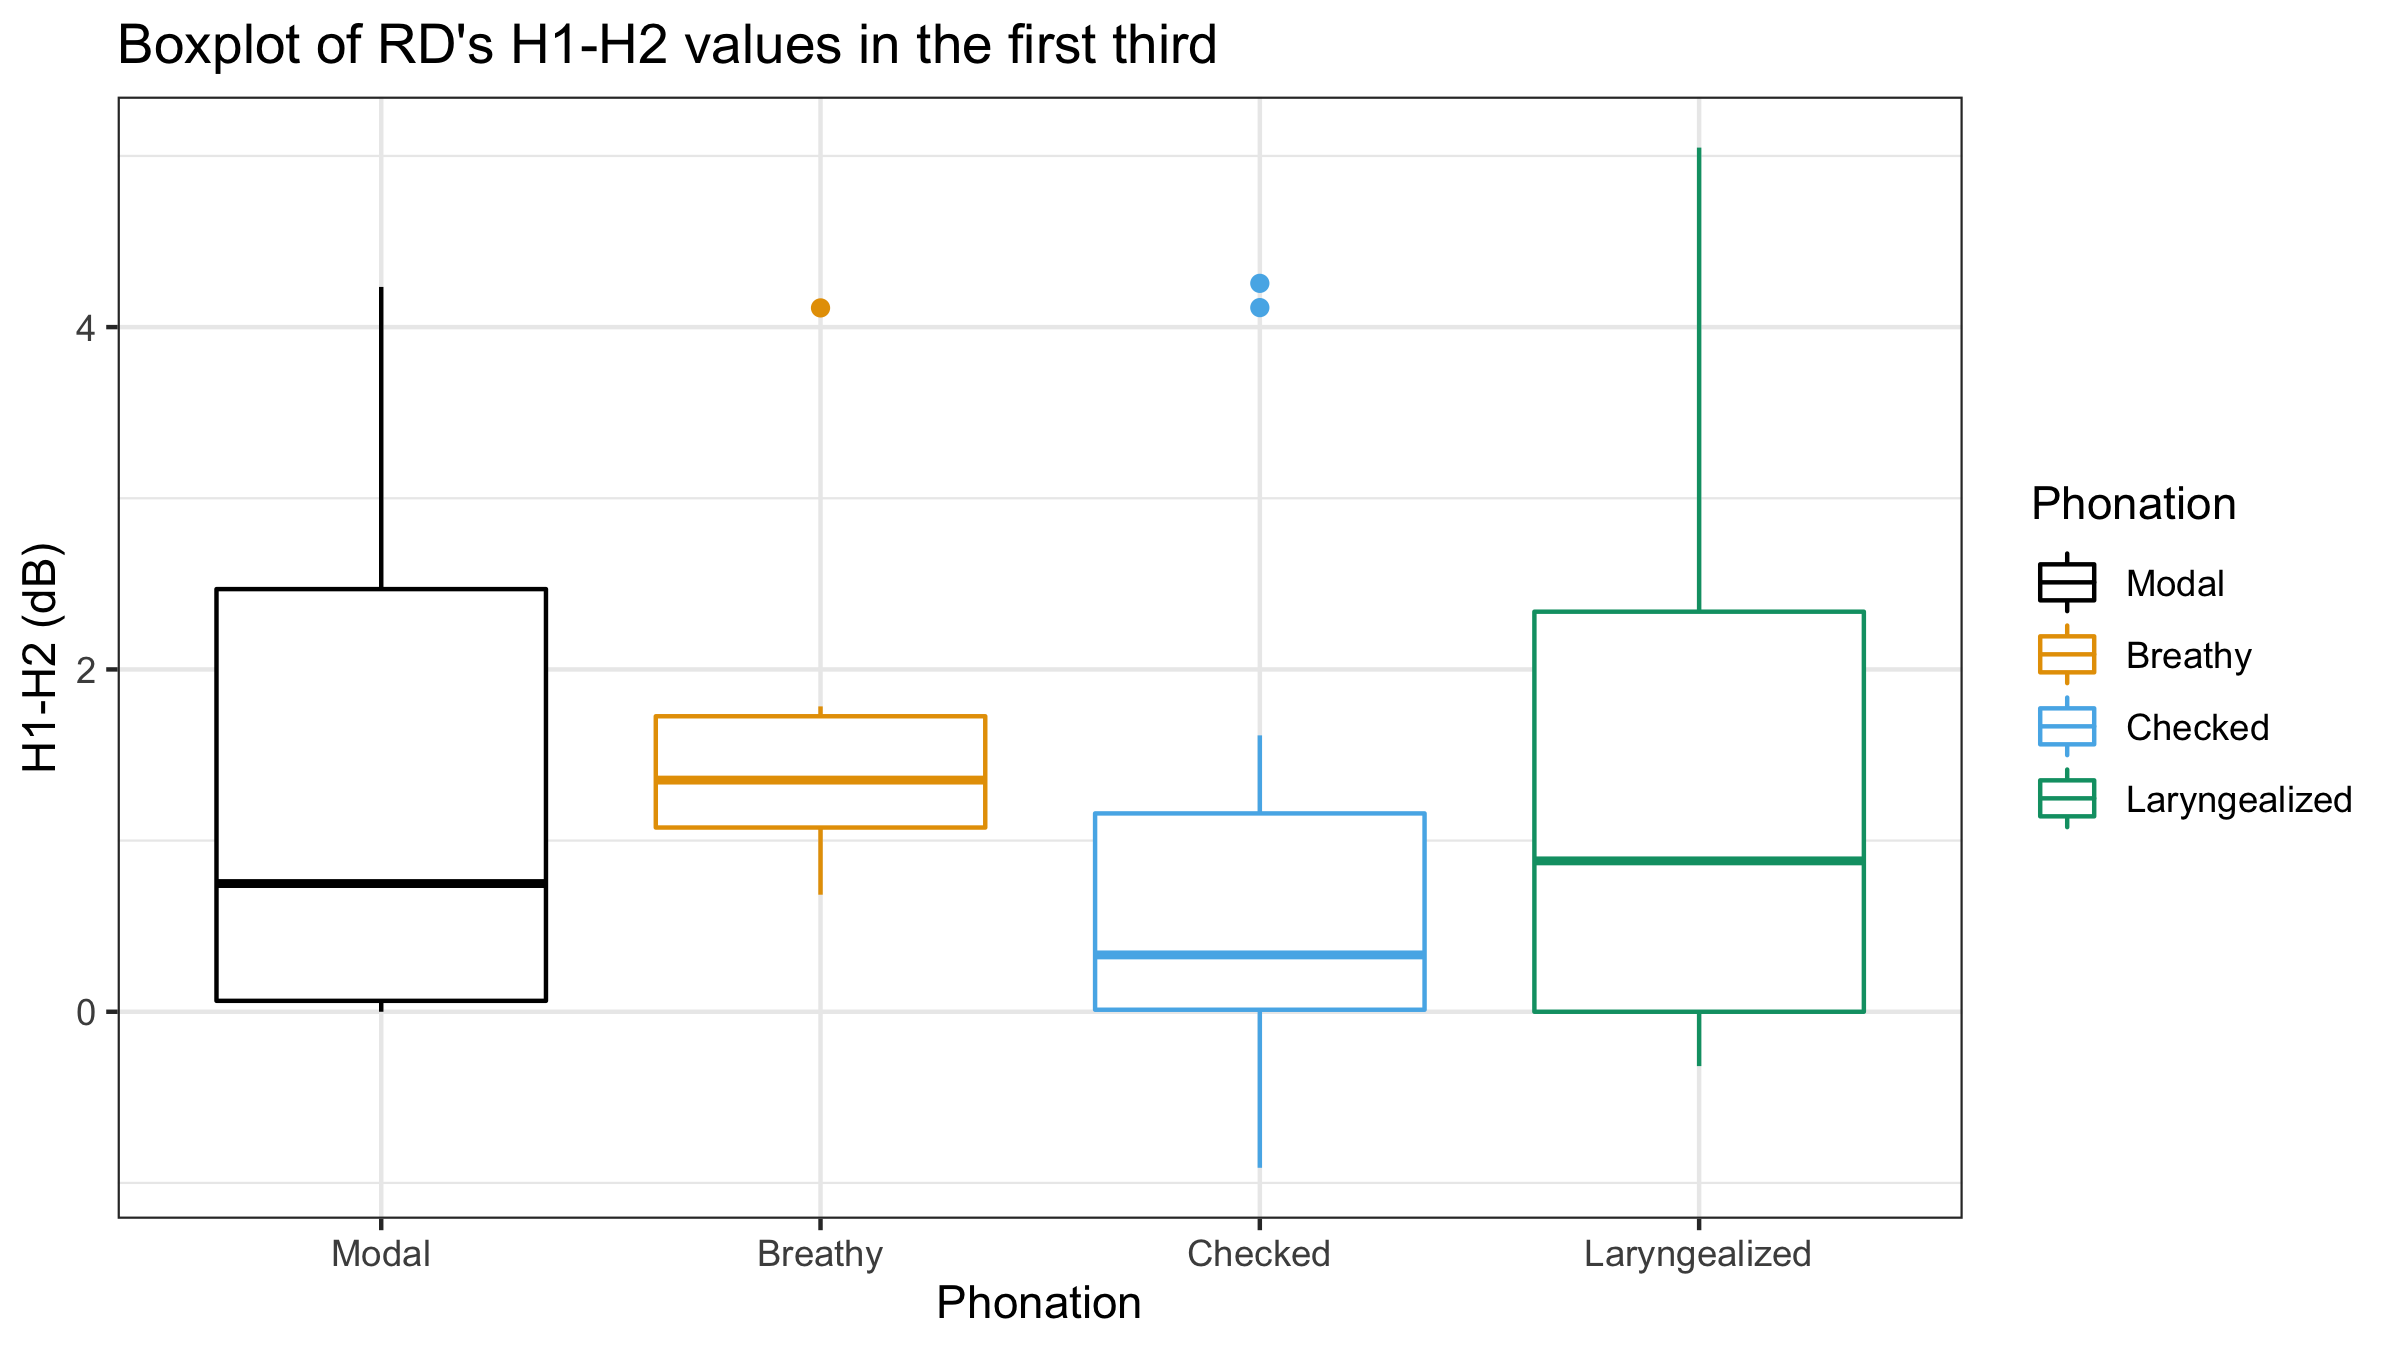
\includegraphics[width=0.9\textwidth]{../mean_RD_h1h2_1st.png}
		\caption{RD's H1-H2 values.}
		\label{fig:RDh1h2first} 
	\end{subfigure}
	\caption{Mean H1-H2 values for the first third of the vowel according to each phonation type. }
	\label{fig:h1h2first}
\end{figure}

\begin{itemize}
	\item Beginning in the second third of the vowel and continuing throughout the vowel, the H1-H2 values for breathy voice is lower than the other three phonation types, which is the opposite of what we expect for breathy voice, see Figure~\ref{fig:h1h2second} for the second third and Figure~\ref{fig:h1h2third} for the final third. 
\end{itemize}

\begin{figure}[!h]
	\centering
	\begin{subfigure}{.5\textwidth}
		\centering
		\includegraphics[width=0.9\textwidth]{../mean_FSR_h1h2_2nd.png}
		\caption{FSR's H1-H2 values.}
		\label{fig:FSRh1h2second} 
	\end{subfigure}%
	\begin{subfigure}{.5\textwidth}
		\centering
		\includegraphics[width=0.9\textwidth]{../mean_RD_h1h2_2nd.png}
		\caption{RD's H1-H2 values.}
		\label{fig:RDh1h2second} 
	\end{subfigure}
	\caption{Mean H1-H2 values for the second third of the vowel according to each phonation type.}
	\label{fig:h1h2second}
\end{figure}

\begin{figure}[!h]
	\centering
	\begin{subfigure}{.5\textwidth}
		\centering
		\includegraphics[width=0.9\textwidth]{../mean_FSR_h1h2_3rd.png}
		\caption{FSR's H1-H2 values.}
		\label{fig:FSRh1h2third} 
	\end{subfigure}%
	\begin{subfigure}{.5\textwidth}
		\centering
		\includegraphics[width=0.9\textwidth]{../mean_RD_h1h2_3rd.png}
		\caption{RD's H1-H2 values.}
		\label{fig:RDh1h2third} 
	\end{subfigure}
	\caption{Mean H1-H2 values for the final third of the vowel according to each phonation type. }
	\label{fig:h1h2third}
\end{figure}
%------------------------------------
\subsection{H1-A3 spectral-tilt results} \label{sec:H1A3}
%------------------------------------

\begin{itemize}
	\item When we consider H1-A3, the measurement \citet{espositoVariationContrastivePhonation2010} found useful for male Zapotec speakers, several observations become apparent. 
	\item In all portions of the vowel, breathy voice shows a much higher H1-A3 measurement than modals as observed in Figures~\ref{fig:h1a3first}, \ref{fig:h1a3second}, and \ref{fig:h1a3third}.
	\item This high H1-A3 value in both speakers is what we expect for breathy vowels \citep{fischer-jorgensenPhoneticAnalysisBreathy1968}. 
\end{itemize}
\begin{figure}[!h]
	\centering
	\begin{subfigure}{.5\textwidth}
		\centering
		\includegraphics[width=0.9\textwidth]{../mean_FSR_h1a3_First.png}
		\caption{FSR's H1-A3 values.}
		\label{fig:FSRh1a3first} 
	\end{subfigure}%
	\begin{subfigure}{.5\textwidth}
		\centering
		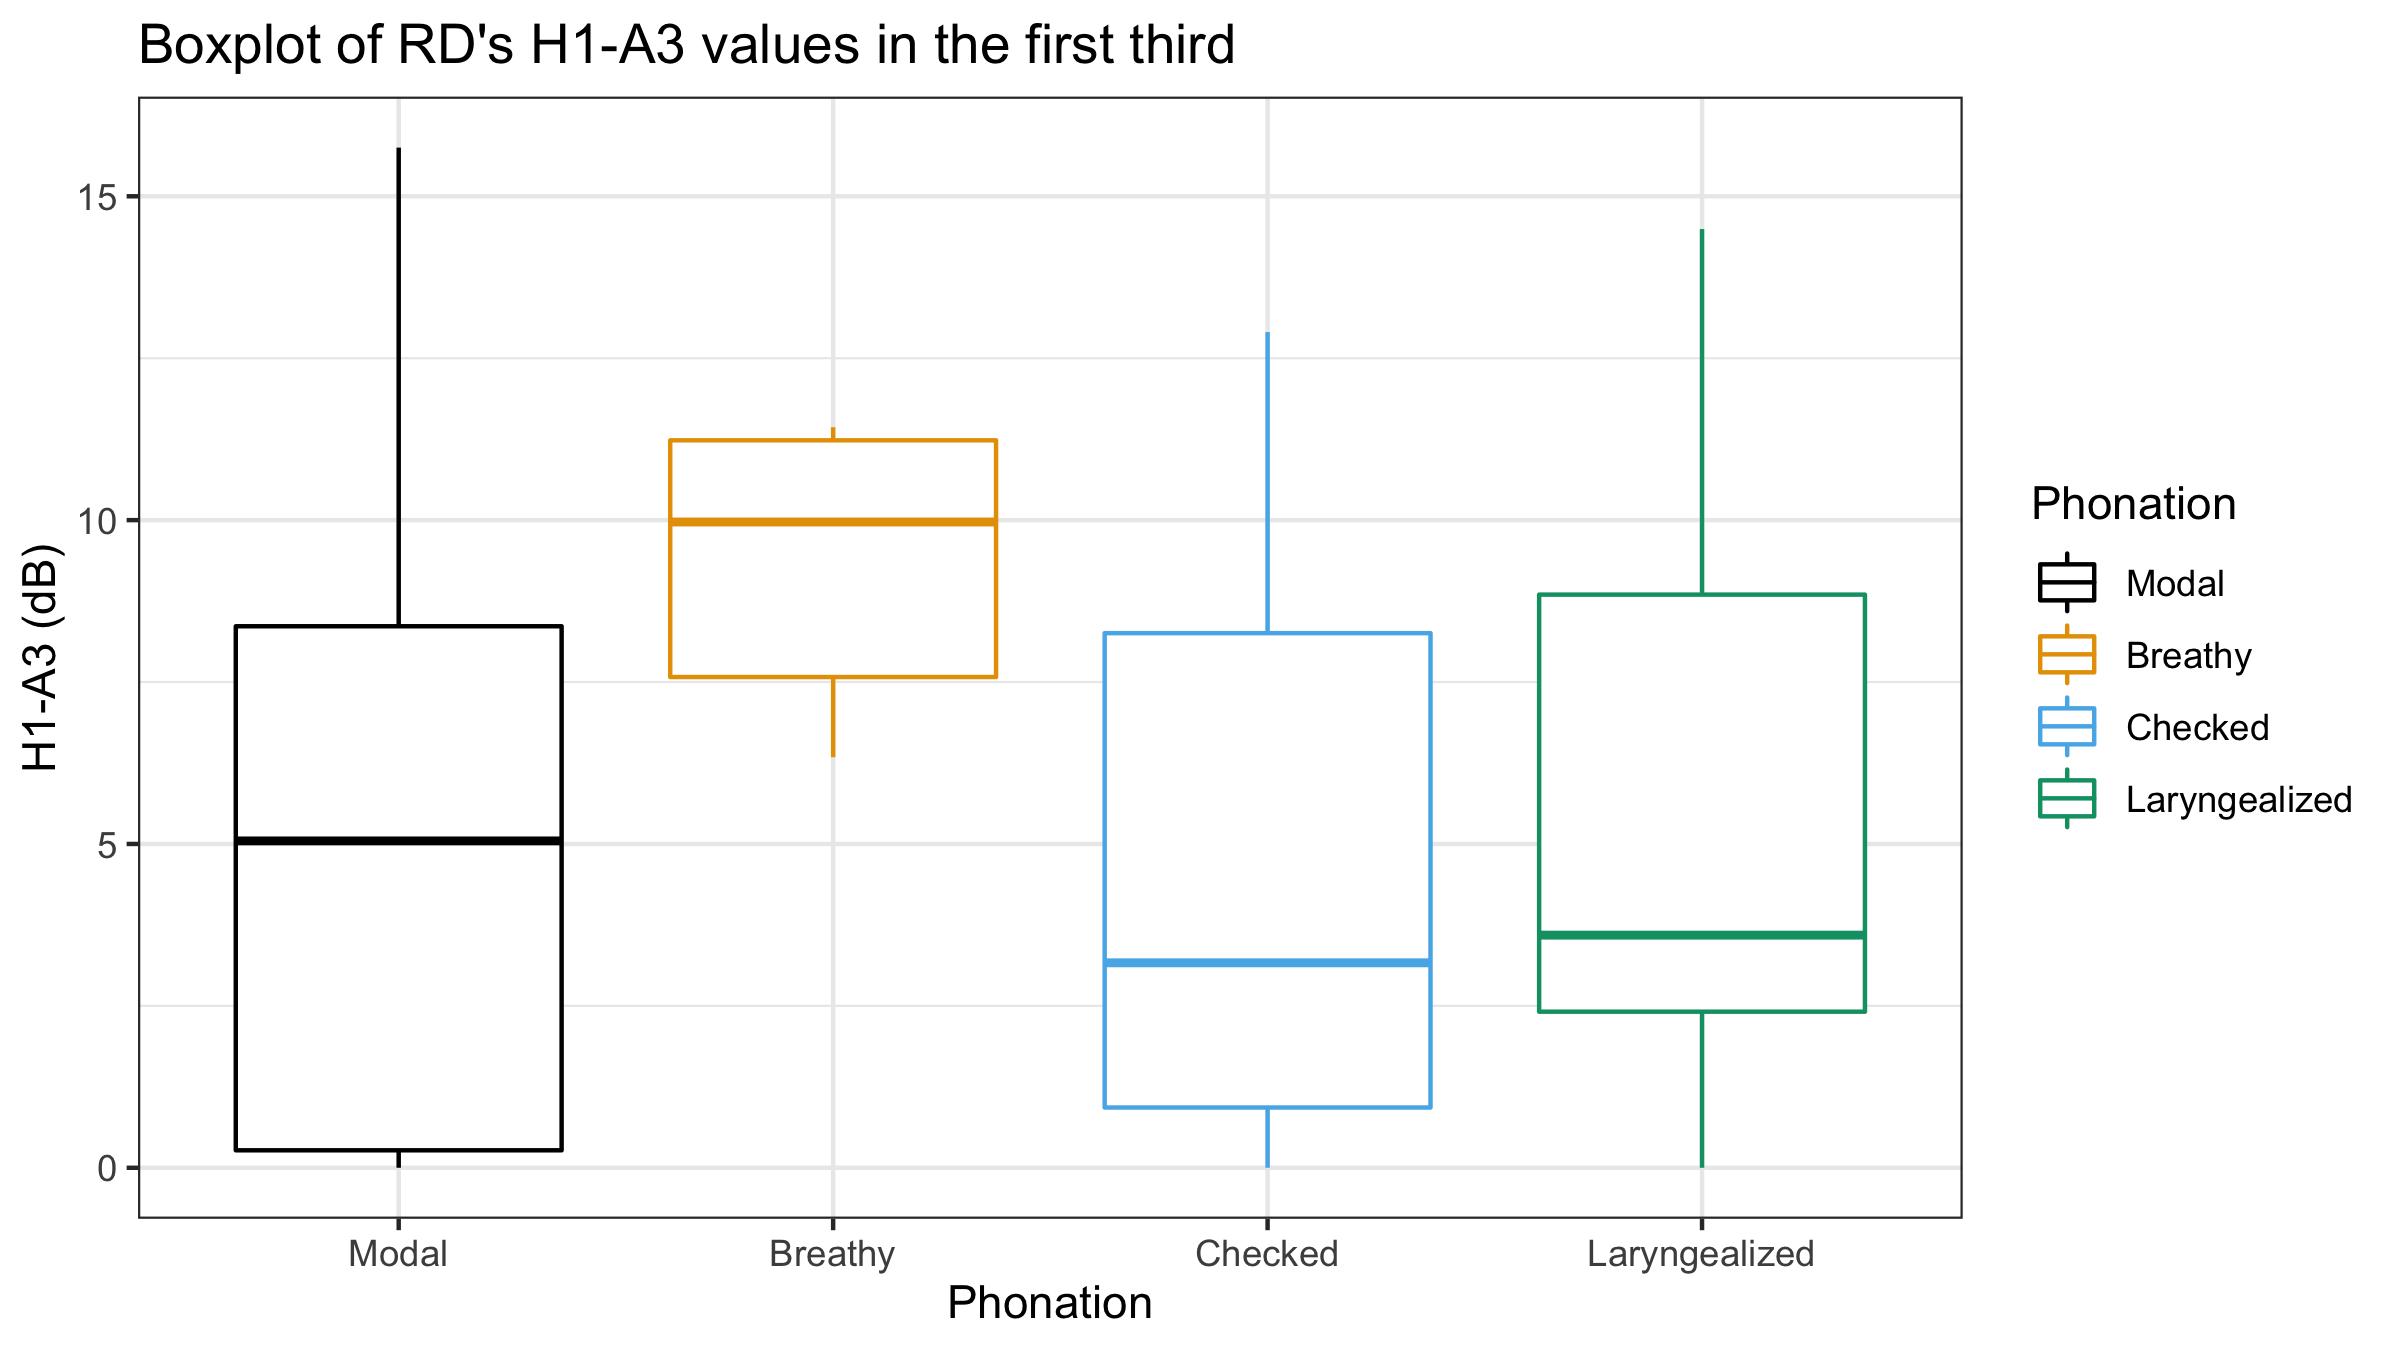
\includegraphics[width=0.9\textwidth]{../mean_RD_h1a3_First.png}
		\caption{RD's H1-A3 values.}
		\label{fig:RDh1a3first} 
	\end{subfigure}
	\caption{H1-A3 values for FSR (a) and RD (b) for the first third of the vowel. }
	\label{fig:h1a3first}
\end{figure}

\begin{itemize}
	\item In Figure~\ref{fig:h1a3first}, we see that there is a large degree of overlap between modals, checked, and laryngealized H1-A3 values. This behavior indicates that there is little to no difference in the phonation types for this portion of the vowel. 
	\item In the second third of the vowel (Figure~\ref{fig:h1a3second}), we see that the checked and laryngealized vowels H1-A3 values for FSR are uninformative because of the large degree of overlap.
	\item Beginning in the middle of the vowel and continuing throughout the rest of the vowel, RD shows a lower H1-A3 value in the laryngealized vowels than the modals which is consistent with creakier productions of vowels, see Figure~\ref{fig:RDh1a3second} and Figure~\ref{fig:RDh1a3third}.
	\item In both speakers there is no difference between modal and creaky for the middle third of the vowel. 
\end{itemize}
\begin{figure}[!h]
	\centering
	\begin{subfigure}{.5\textwidth}
		\centering
		\includegraphics[width=0.9\textwidth]{../mean_FSR_h1a3_Second.png}
		\caption{FSR's H1-A3 values.}
		\label{fig:FSRh1a3second} 
	\end{subfigure}%
	\begin{subfigure}{.5\textwidth}
		\centering
		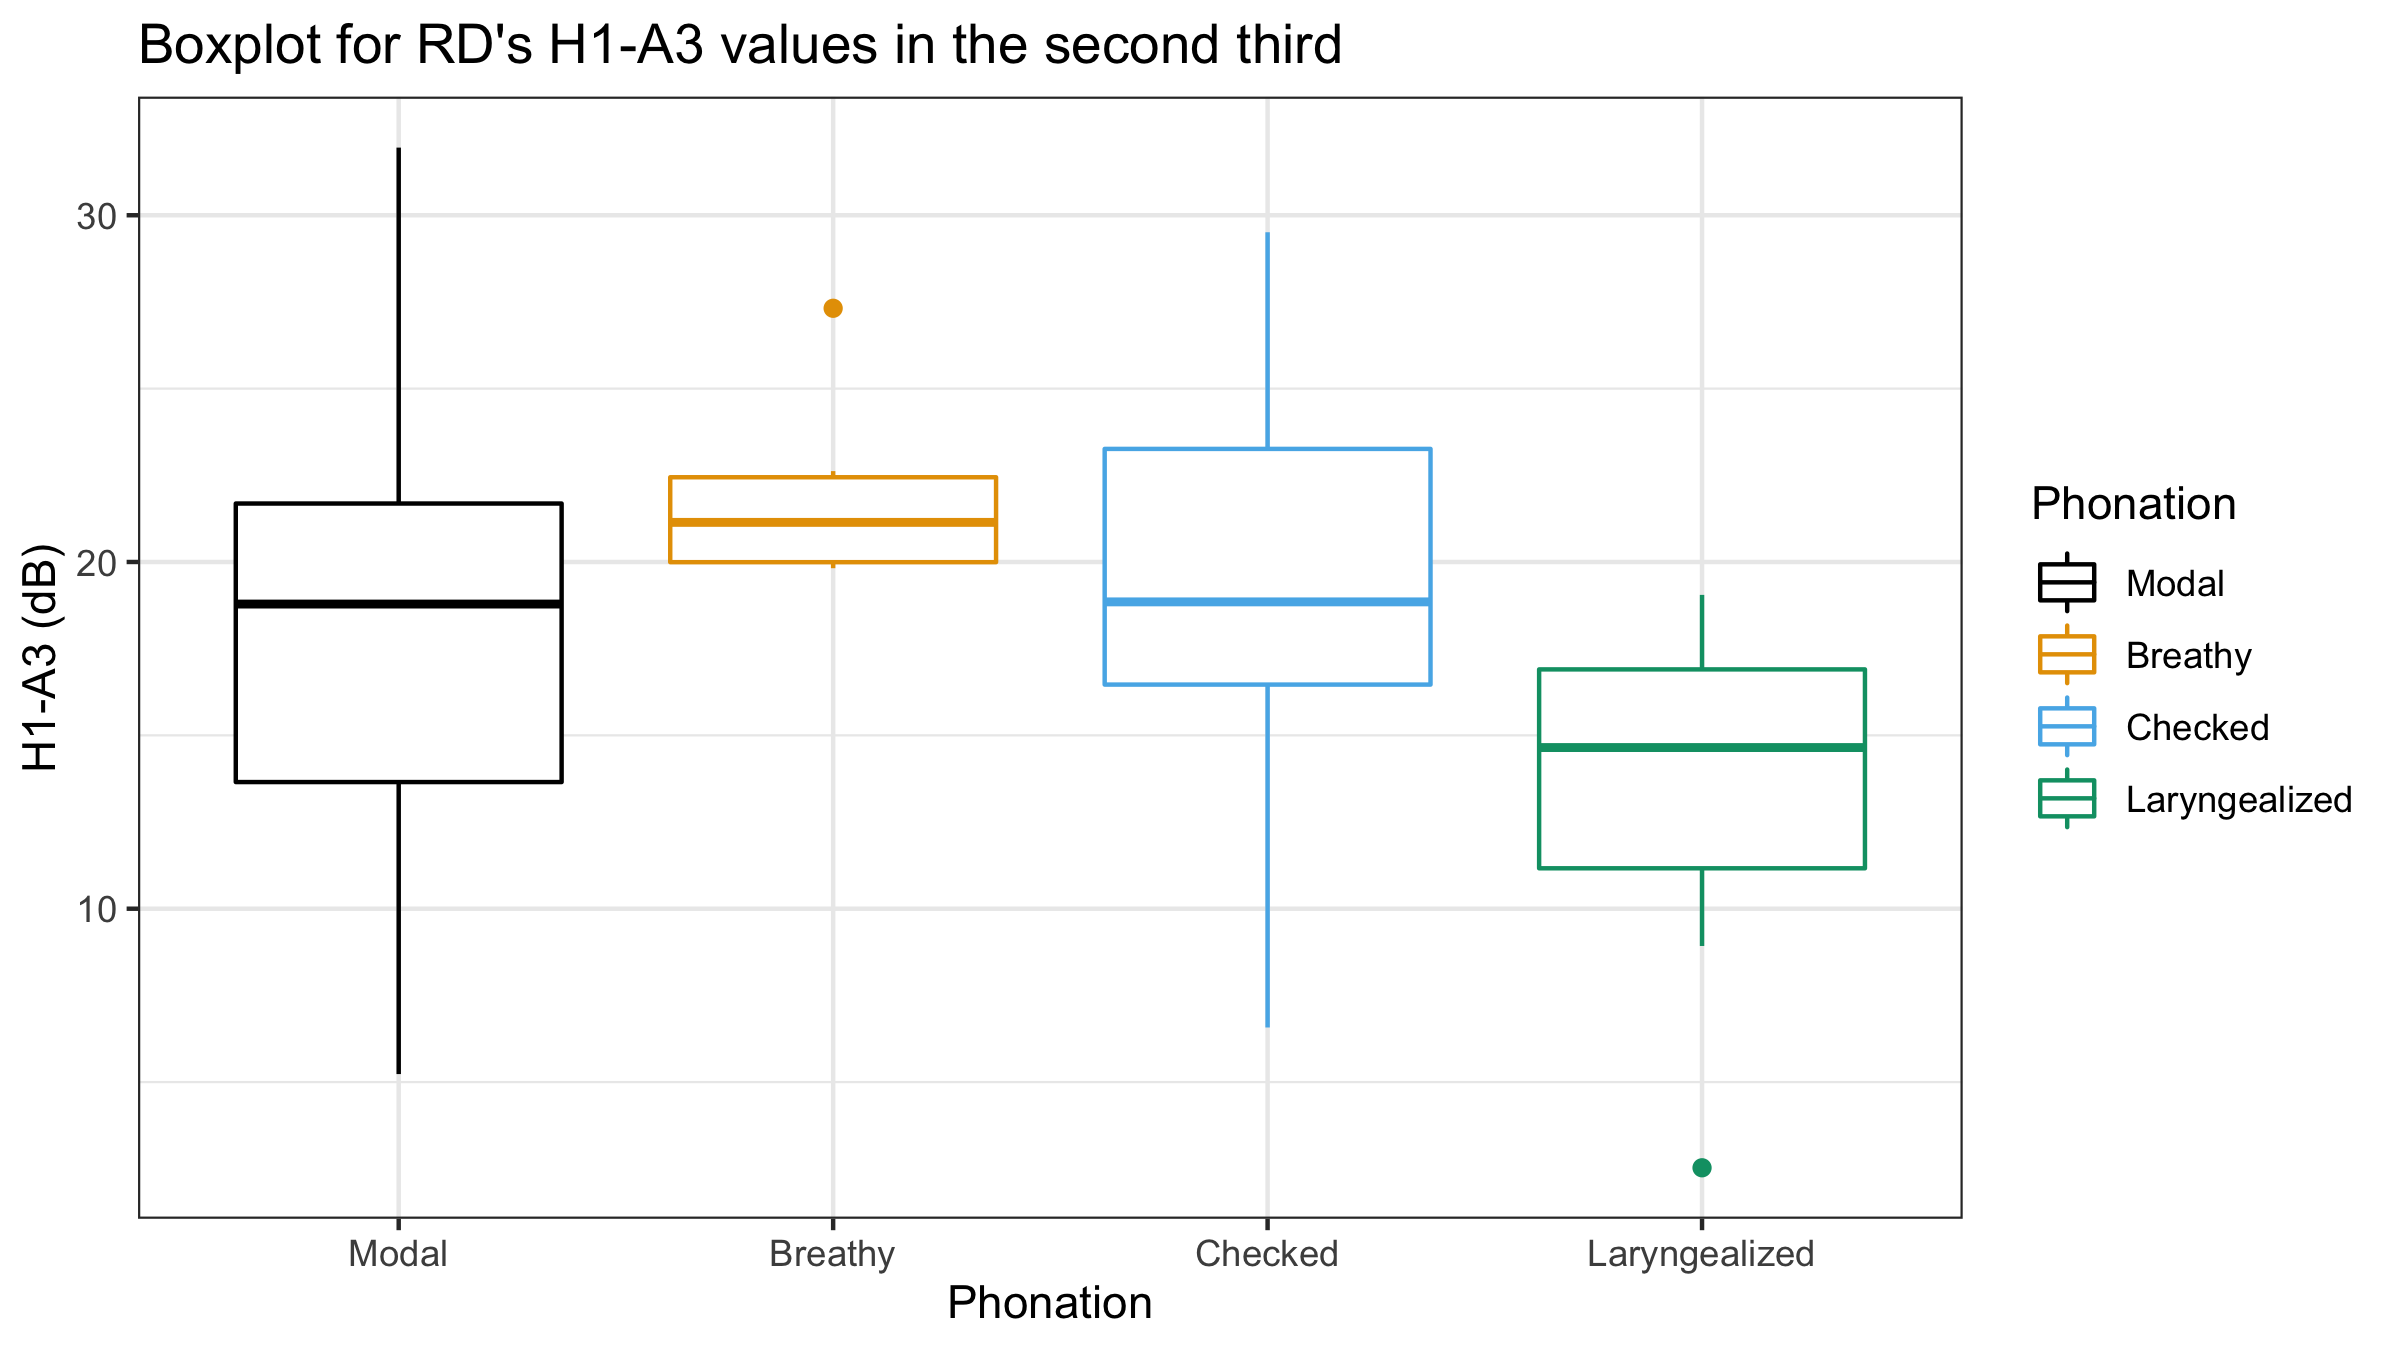
\includegraphics[width=0.9\textwidth]{../mean_RD_h1a3_Second.png}
		\caption{RD's H1-A3' values.}
		\label{fig:RDh1a3second} 
	\end{subfigure}
	\caption{H1-A3 values for FSR (a) and RD (b) for the second third of the vowel. }
	\label{fig:h1a3second}
\end{figure}

\begin{itemize}
	\item In the final third of the vowel, FSR's production of checked vowels show a lower H1-A3 measurement, which suggests FSR produces a period of creakiness in the last third of these vowels. 
	\item For RD, however, there are no differences between checked and modal vowels in this last third. 
\end{itemize}

\begin{figure}[!h]
	\centering
	\begin{subfigure}{.5\textwidth}
		\centering
		\includegraphics[width=0.9\textwidth]{../mean_FSR_h1a3_third.png}
		\caption{FSR's H1-A3 values.}
		\label{fig:FSRh1a3third} 
	\end{subfigure}%
	\begin{subfigure}{.5\textwidth}
		\centering
		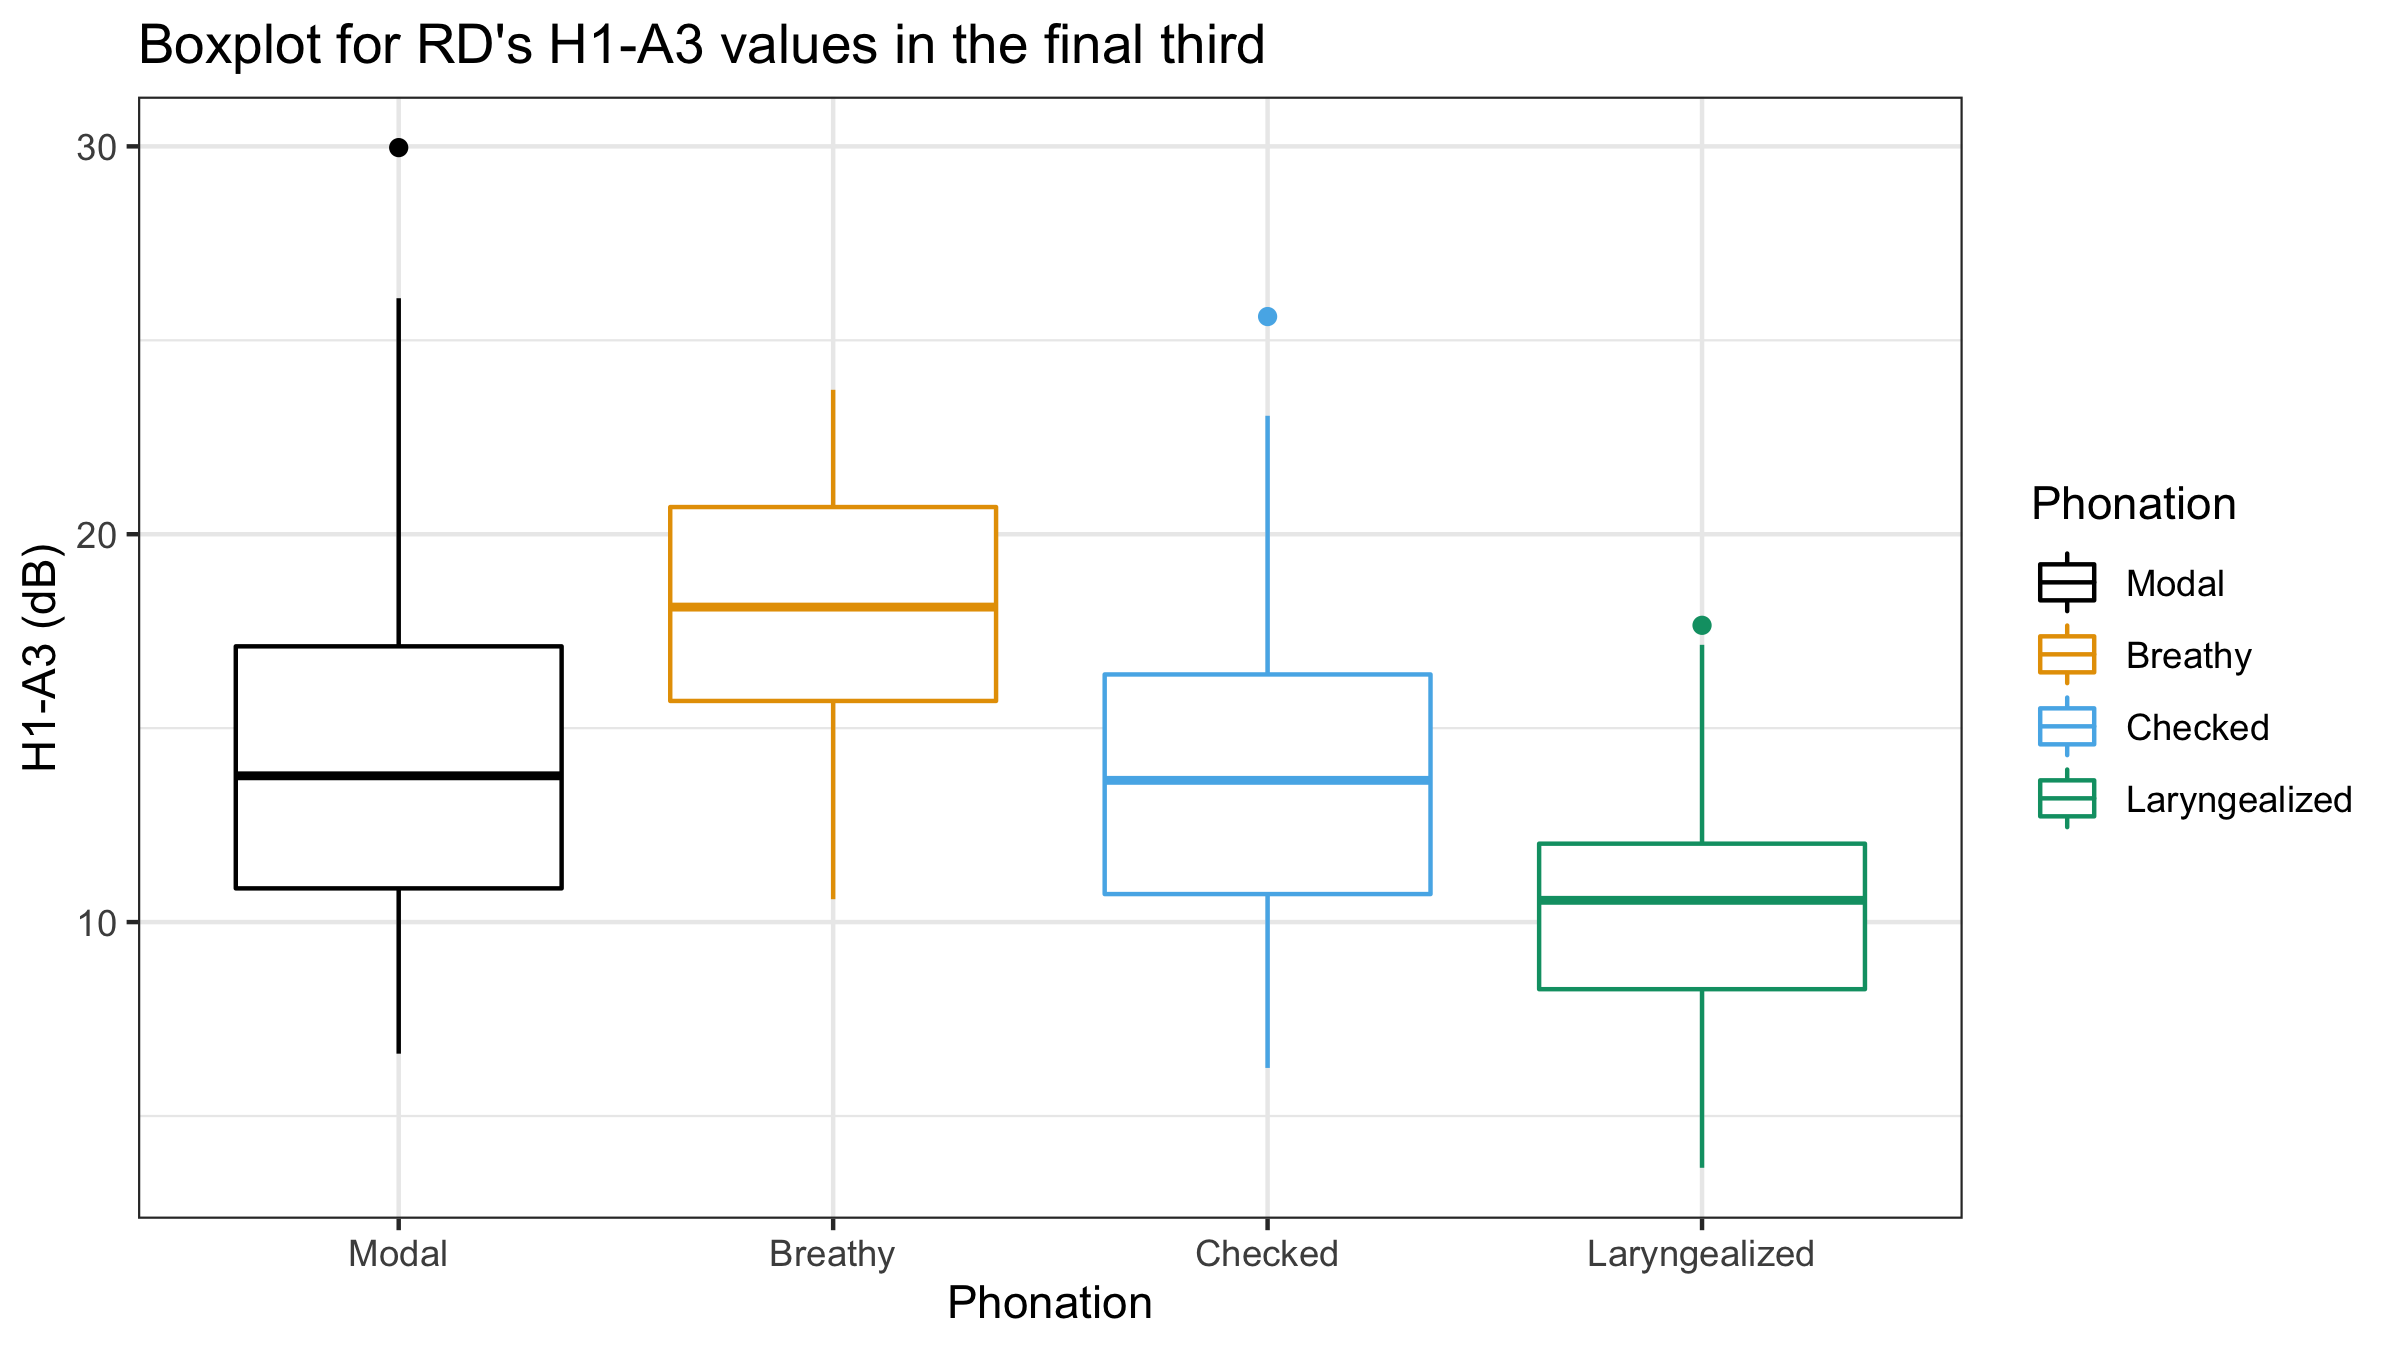
\includegraphics[width=0.9\textwidth]{../mean_RD_h1a3_third.png}
		\caption{RD's H1-A3 values.}
		\label{fig:RDh1a3third} 
	\end{subfigure}
	\caption{H1-A3 values for FSR (a) and RD (b) for the final third of the vowel. }
	\label{fig:h1a3third}
\end{figure}

%------------------------------------
\subsection{Cepstral Peak Prominence results} \label{sec:CPP}
%------------------------------------

\begin{itemize}
	\item In determining if there is any amount of aperiodicity in the signal, we turn to CPP \citep{hillenbrandAcousticCorrelatesBreathy1994,hillenbrandAcousticCorrelatesBreathy1996}.
	\item A CPP measurement for any vowel with non-modal phonation should be lower than the CPP
	measurement for modal vowels.
	\item Throughout the whole vowel, CPP measures for both FSR and RD are consistently higher for breathy vowels than modal vowels. 
	\item This observation seems to suggest that breathy vowels are in some way more periodic than modal vowels. 
\end{itemize}
\begin{figure}[!h]
	\centering
	\begin{subfigure}{.5\textwidth}
		\centering
		\includegraphics[width=0.9\textwidth]{../mean_FSR_cpp_First.png}
		\caption{FSR's CPP values.}
		\label{fig:FSRcppfirst} 
	\end{subfigure}%
	\begin{subfigure}{.5\textwidth}
		\centering
		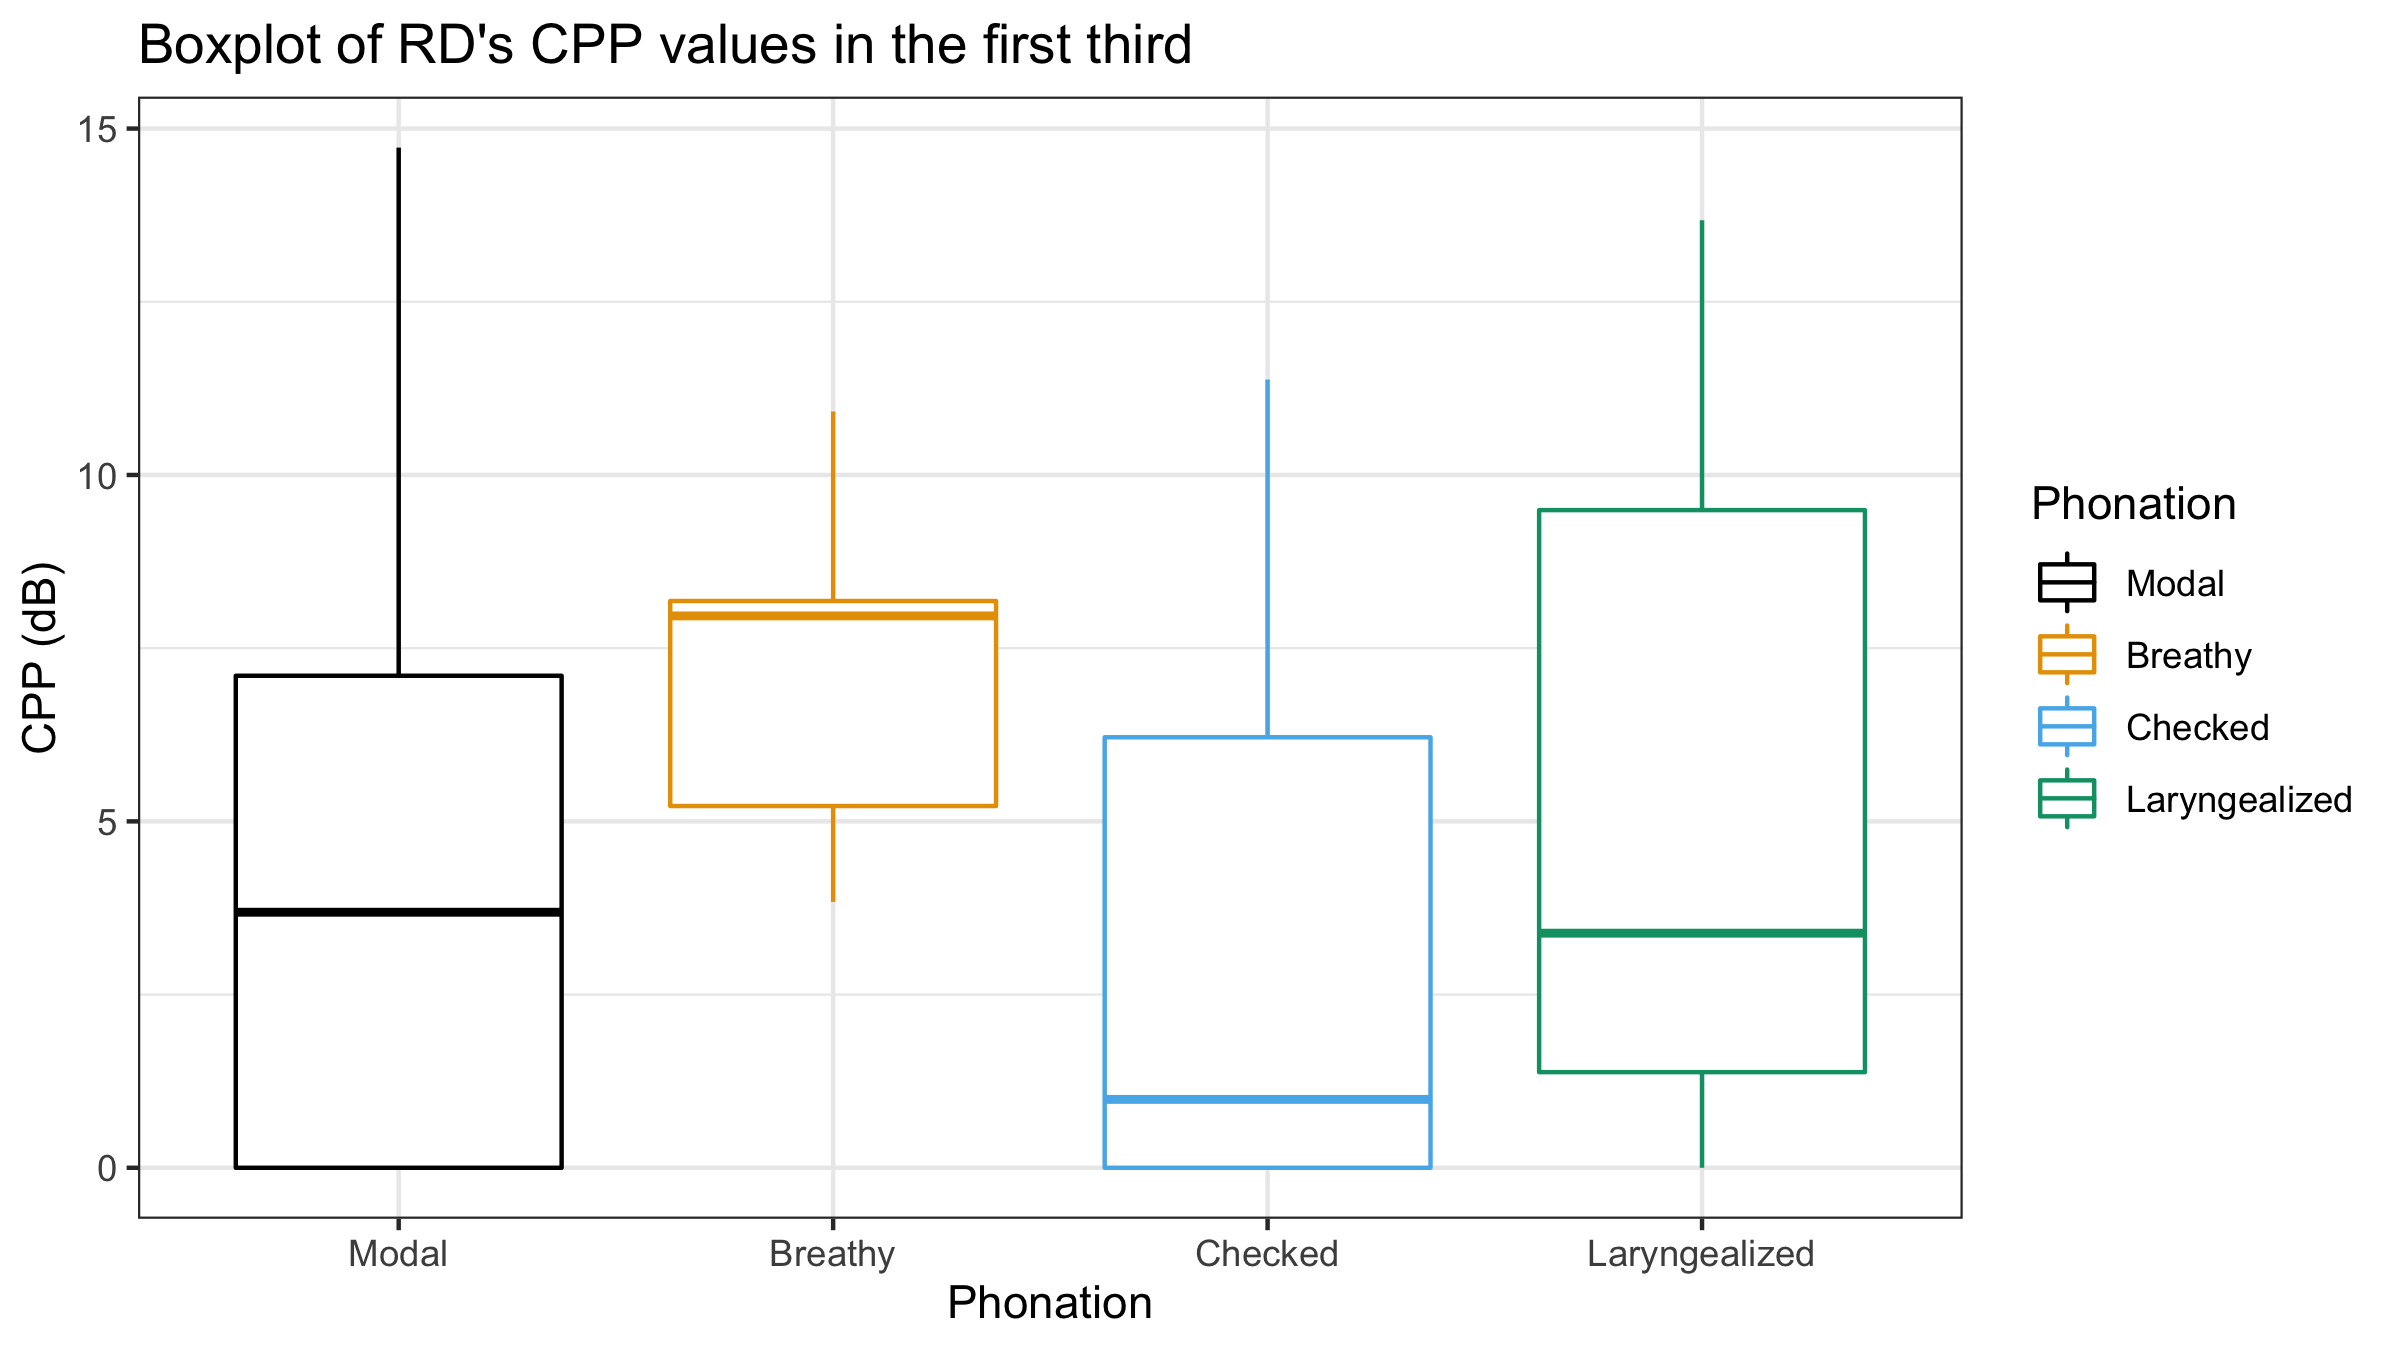
\includegraphics[width=0.9\textwidth]{../mean_RD_cpp_First.png}
		\caption{RD's CPP values.}
		\label{fig:RDcppfirst} 
	\end{subfigure}
	\caption{CPP values for FSR (a) and RD (b) for the first third of the vowel. }
	\label{fig:cppfirst}
\end{figure}

\begin{itemize}
	\item When we turn to the middle third of the vowel, Figure~\ref{fig:cppsecond}, we observe that FSR's laryngealized vowels show a lower CPP value, indicating that there is aperiodicity in this portion of the vowel. 
	\item For RD, there are no differences between modal, breathy, or checked in this portion of the vowel. 
\end{itemize}
\begin{figure}[!h]
	\centering
	\begin{subfigure}{.5\textwidth}
		\centering
		\includegraphics[width=0.9\textwidth]{../mean_FSR_cpp_Second.png}
		\caption{FSR's CPP values.}
		\label{fig:FSRcppsecond} 
	\end{subfigure}%
	\begin{subfigure}{.5\textwidth}
		\centering
		\includegraphics[width=0.9\textwidth]{../mean_RD_cpp_Second.png}
		\caption{RD's CPP values.}
		\label{fig:RDcppsecond} 
	\end{subfigure}
	\caption{CPP values for FSR (a) and RD (b) for the second third of the vowel. }
	\label{fig:cppsecond}
\end{figure}

\begin{itemize}
	\item In both FSR and RD, we observe a lower CPP value for checked vowels in the final third of the vowel. 
	\item This is consistent with a period of aperiodicity at the end of the vowel. 
\end{itemize}
\begin{figure}[!h]
	\centering
	\begin{subfigure}{.5\textwidth}
		\centering
		\includegraphics[width=0.9\textwidth]{../mean_FSR_cpp_third.png}
		\caption{FSR's CPP values.}
		\label{fig:FSRcppthird} 
	\end{subfigure}%
	\begin{subfigure}{.5\textwidth}
		\centering
		\includegraphics[width=0.9\textwidth]{../mean_RD_cpp_third.png}
		\caption{RD's CPP values.}
		\label{fig:RDcppthird} 
	\end{subfigure}
	\caption{CPP values for FSR (a) and RD (b) for the final third of the vowel. }
	\label{fig:cppthird}
\end{figure}

%------------------------------------
\subsection{Statistical results} \label{sec:Stats}
%------------------------------------
\begin{itemize}
	\item In order to determine whether or not the different acoustic measurements were effective at capturing the different phonation types, a mixed-effects linear regression analysis was performed
	with a Satterthwaite’s method for t-test analysis used to derive the p-values. 
	\item Each of different measurements were treated as the dependent variable with word and speaker treated as random.
\end{itemize}

%------------------------------------
\subsubsection{H1-H2 statistical results} \label{sec:StatsH1H2}
%------------------------------------

\begin{itemize}
	\item As can be recalled from Section~\ref{sec:H1H2}, both FSR and RD show a lower value for H1-H2 for breathy vowels in the last two-thirds of the vowels when compared to the model vowel's H1-H2 values. 
	\item The results of the statistical analysis for the last two-thirds of the vowel, presented in Table~\ref{tab:H1H2_Second} and Table~\ref{tab:H1H2_Third}, show that this behavior is significant.
	\item At no point do the other phonation types reach significance with respect to H1-H2. 
\end{itemize}

\begin{table}[!h]
	\centering
	\caption{Results of the mixed-effects linear regression analysis on the first third of the vowel for H1-H2. }
	\label{tab:H1H2_First}
	 \begin{tabular}{llllll}
	  \lsptoprule
						&  Estimate  & Std. Error & df & t value & p-value \\
	  	Breathy   		&  -0.3049  &   0.5795 & 116.4255 &  -0.526  &  0.600 \\
		Checked    		&  -0.4731  &   0.4029 & 145.6184 &  -1.174  &  0.242 \\
		Laryngealized	&  -0.2938  &   0.4675 & 101.9977 &  -0.629  &  0.531 \\
	  \lspbottomrule
	 \end{tabular}
\end{table}

\begin{table}[!h]
	\centering
	\caption{Results of the mixed-effects linear regression analysis on the second third of the vowel for H1-H2. }
	\label{tab:H1H2_Second}
	 \begin{tabular}{llllll}
	  \lsptoprule
						&  Estimate  & Std. Error & df & t value & p-value \\
	  	Breathy   		&  -3.4158  &   1.3400 & 126.9590 &  -2.549  &  0.0120 \\
		Checked    		&  -1.7466  &   0.9197 & 146.9995 &  -1.899  &  0.0595 \\
		Laryngealized	&  -0.7405  &   1.0852 & 117.0669 &  -0.682  &  0.4963 \\
	  \lspbottomrule
	 \end{tabular}
\end{table}

\begin{table}[!h]
	\centering
	\caption{Results of the mixed-effects linear regression analysis on the final third of the vowel for H1-H2. }
	\label{tab:H1H2_Third}
	 \begin{tabular}{llllll}
	  \lsptoprule
						&  Estimate  & Std. Error & df & t value & p-value \\
	  	Breathy   		&  -2.2131  &   1.0291 & 125.2092 &  -2.151  &  0.0334 \\
		Checked    		&  -1.3487  &   0.6952 & 146.2461 &  -1.940  &  0.0543 \\
		Laryngealized	&  -0.8676  &   0.8202 & 116.8963 &  -1.058  &  0.2923 \\
	  \lspbottomrule
	 \end{tabular}
\end{table}

%------------------------------------
\subsubsection{H1-A3 statistical results} \label{sec:StatsH1A3}
%------------------------------------

\begin{itemize}
	\item The second statistical analysis for the H1-A3 measurement shows some very clear behavior for breathy voice. 
	\item In Section~\ref{sec:H1A3} we observe that breathy voice is clearly identified in all portions of the vowel with an elevated H1-A3 value when compared to modals. 
	\item We see that for all portions of the vowel, as seen in Tables~\ref{tab:H1A3_First}, \ref{tab:H1A3_Second}, \ref{tab:H1A3_Third} breathy voice reaches significance.
\end{itemize}
  
\begin{table}[!h]
	\centering
	\caption{Results of the mixed-effects linear regression analysis on the first third of the vowel for H1-A3. }
	\label{tab:H1A3_First}
	 \begin{tabular}{llllll}
	  \lsptoprule
						&  Estimate  & Std. Error & df & t value & p-value \\
	  	Breathy   		&  4.29036  &  1.31288 & 137.12067 &  3.268  &  0.00137\\
		Checked    		&  0.15001  &  0.84476 & 134.62215 &  0.178  &  0.85932 \\
		Laryngealized	& -0.05694  &  1.07130 & 137.16596 & -0.053  &  0.95769\\
	  \lspbottomrule
	 \end{tabular}
\end{table}

\begin{itemize}
	\item When corrected for word and speaker, laryngealized vowels reach significance in the second third of the vowel. 
\end{itemize}

\begin{table}[!h]
	\centering
	\caption{Results of the mixed-effects linear regression analysis on the second third of the vowel for H1-A3. }
	\label{tab:H1A3_Second}
	 \begin{tabular}{llllll}
	  \lsptoprule
						&  Estimate  & Std. Error & df & t value & p-value \\
	  	Breathy   		&  4.398    &  2.027 & 147.003 &  2.169 &  0.0317 \\
		Checked    		&  1.195    &  1.426 & 147.000 &  0.838 &  0.4033  \\
		Laryngealized	& -2.694    &  1.627 & 147.001 & -1.656 &  0.0998 \\
	  \lspbottomrule
	 \end{tabular}
\end{table}

\begin{itemize}
	\item In the final third of the vowel, H1-A3 was only significant for breathy voice. 
\end{itemize}

\begin{table}[!h]
	\centering
	\caption{Results of the mixed-effects linear regression analysis on the final third of the vowel for H1-A3. }
	\label{tab:H1A3_Third}
	 \begin{tabular}{llllll}
	  \lsptoprule
						&  Estimate  & Std. Error & df & t value & p-value \\
	  	Breathy   		&  5.2928   &  1.7966 & 127.0400 &  2.946 & 0.00383 \\
		Checked    		& -0.7825   &  1.2487 & 147.1011 & -0.627 & 0.53189 \\
		Laryngealized	& 0.2669    &  1.4224 & 117.4917 &  0.188 & 0.85151 \\
	  \lspbottomrule
	 \end{tabular}
\end{table}

%------------------------------------
\subsubsection{CPP statistical results} \label{sec:StatsCPP}
%------------------------------------

\begin{itemize}
	\item When we consider CPP, we see that this measurement was significant for all three of the phonation types but in different portions of the vowel. 
	\item In Table~\ref{tab:CPP_First}, we see that the high CPP values observed in Section~\ref{sec:CPP} for the first third of the vowel was significant. 
	\item For checked and laryngealized vowels CPP fails to reach significance in this first third. 
\end{itemize}

\begin{table}[!h]
	\centering
	\caption{Results of the mixed-effects linear regression analysis on the first third of the vowel for CPP. }
	\label{tab:CPP_First}
	 \begin{tabular}{llllll}
	  \lsptoprule
						&  Estimate  & Std. Error & df & t value & p-value \\
	  	Breathy   		&  3.4470   &  1.1743 & 145.9760 &  2.935 & 0.00387 \\
		Checked    		& -1.4190   &  0.7088 & 120.5020 & -2.002 & 0.04754 \\
		Laryngealized	&  0.8240   &  0.9530 & 147.0083 &  0.865 & 0.38868 \\
	  \lspbottomrule
	 \end{tabular}
\end{table}

\begin{itemize}
	\item In the middle of the vowel, only laryngealized voice was significant, see Table~\ref{tab:CPP_Second}. 
\end{itemize}


\begin{table}[!h]
	\centering
	\caption{Results of the mixed-effects linear regression analysis on the second third of the vowel for CPP. }
	\label{tab:CPP_Second}
	 \begin{tabular}{llllll}
	  \lsptoprule
						&  Estimate  & Std. Error & df & t value & p-value \\
	  	Breathy   		&  1.5044   &  1.4073 & 128.0083 &  1.069 & 0.287094 \\
		Checked    		& -0.5804   &  0.9789 & 146.0792 & -0.593 & 0.554154 \\
		Laryngealized	& -2.2898   &  1.1354 & 117.6213 & -2.017 & 0.046006 \\
	  \lspbottomrule
	 \end{tabular}
\end{table}

\begin{itemize}
	\item In the final portion of the vowel, Table~\ref{tab:CPP_Third}, only the CPP values for checked phonation reached significance.
\end{itemize}

\begin{table}[!h]
	\centering
	\caption{Results of the mixed-effects linear regression analysis on the final third of the vowel for CPP. }
	\label{tab:CPP_Third}
	 \begin{tabular}{llllll}
	  \lsptoprule
						&  Estimate  & Std. Error & df & t value & p-value \\
	  	Breathy   		&  1.6391   &  1.0173  & 139.8563 &  1.611 & 0.10939 \\
		Checked    		& -2.1386   &  0.6449  & 129.1392 & -3.316 & 0.00119 \\
		Laryngealized	& -1.1158   &  0.8142  & 140.5570 & -1.370 & 0.17274\\
	  \lspbottomrule
	 \end{tabular}
\end{table}

%------------------------------------
\section{Discussion} \label{sec:Discussion}
%------------------------------------

%------------------------------------
\subsection{Acoustics discussion} \label{sec:Acoustics}
%------------------------------------

%------------------------------------
\subsubsection{H1-H2 discussion} \label{sec:DiscH1H2}
%------------------------------------

\begin{itemize}
	\item Overall, H1-H2 was uninformative for phonation in SLZ. 
	\item This is in contrast to \citet{adlerAcousticsPhonationTypes2016} which found for two male speakers of SLZ H1-H2 was informative. 
	\item This difference could be attributed to a hypothesis put forward by \citet{espositoVariationContrastivePhonation2010} that maybe the speakers are producing the phonation types differently than the speakers in this study. 
	\item Additionally, \citet{chaiH1H2Acoustic2022} remark that there is a growing body of evidence that H1-H2 is not a reliable measure of phonation.
	\item \citet{sundbergObjectiveCharacterizationPhonation2022} found that this unreliability is because H2 can be highly influenced by differences in subglottal pressure. 
	\item More specifically, H2 is more sensitive to the pulse amplitude increase than H1. 
	\item This sensitivity results in an inverse relationship between H1-H2 and pulse amplitude.
	\item Furthermore, the results also show that H1-H2 is not a reliable measure in SLZ.
	\item Another question that this raises is whether more speakers were sampled if the results would be different. 
\end{itemize}
%------------------------------------
\subsubsection{H1-A3 discussion} \label{sec:DiscH1H2}
%------------------------------------

\begin{itemize}
	\item H1-A3, however, appears to be a good measure for breathy voice in SLZ for both speakers. 
	\item This shows that, similar to \citet{espositoVariationContrastivePhonation2010}, H1-A3 is a good measure for capturing some of the phonation contrasts in SLZ.
	\item However, unlike \citeauthor{espositoVariationContrastivePhonation2010}, this measure was not informative for creaky or laryngealized voice as indicated by the linear regression.
	\item Similar to H1-A3 it is possible that the results might be different if there was a larger sample pool. 
\end{itemize}

%------------------------------------
\subsubsection{CPP discussion} \label{sec:DiscH1H2}
%------------------------------------
\begin{itemize}
	\item The results of CPP were both informative and concerning. 
	\item Breathy voice, as seen in Section~\ref{sec:CPP} and shown to be significant in Section~\ref{sec:StatsCPP}, the CPP value was much higher for both speakers.
	\item This is the opposite of what we expect to see for periods of aperiodicity \citep{hillenbrandAcousticCorrelatesBreathy1994,hillenbrandAcousticCorrelatesBreathy1996}.
	\item This suggests that breathy vowels were more periodic that modal vowels. 
	\item It is possible that several of the vowels were mislabeled as being modal or breathy when they were actually a different phonation type. 
	\begin{itemize}
		\item This is because it is rather difficult to hear breathy voice when listening to the audio produced by Zencastr. 
		\item It is much easier to hear breathy voice when in person. 
		\item Additionally, when in Laxopa this summer, Maya and I realized that many words had the wrong phonation type associated with them.
	\end{itemize}
	\item With checked and laryngealized voice, we see the drop in CPP we expect to see with aperiodic noise. 
	\item These drops were significant even when correcting for word and speaker
	\item This suggests that aperiodic noise might be the main cue to laryngealized and checked voice for these speakers. 
	\item Additionally, we notice that there is an apparent difference in timing between when this aperiodic noise begins. 
	\begin{itemize}
		\item Laryngealized vowels have this aperiodic noise centered in the middle of the vowel. 
		\item Checked vowel have this aperiodic noise begin in the final third of the vowel. 
	\end{itemize}
	\item This difference in timing is important because both phonation types are associated with creakiness in the vowel. 
	\item This is consistent with the observation that somewhere in the middle of the vowel there is either a full glottal stop or a period of creakiness in the two speakers that were evaluated for this study. 
	\item This observation also bears witness to observations made by \citet{avelinoAcousticElectroglottographicAnalyses2010} about the how each of the different manners that laryngealized vowels are produced in Yalálag Zapotec.
	\item This difference in timing is similar to observations made by \citet{silvermanLaryngealComplexityOtomanguean1997,silvermanPhasingRecoverability1997,blankenshipTimeCourseBreathiness1997,blankenshipTimingNonmodalPhonation2002} for nonmodal phonation in the Laryngeal Complexity Hypothesis.
\end{itemize}


%------------------------------------
\subsection{Laryngeal Complexity Hypothesis} \label{sec:LCH}
%------------------------------------

\begin{itemize}
	\item The Laryngeal Complexity Hypothesis (LCH) has its origin in work from \citet{silvermanLaryngealComplexityOtomanguean1997,blankenshipTimeCourseBreathiness1997,blankenshipTimingNonmodalPhonation2002}.
	\item The LCH claims that languages that have both tone and phonation need them to be phased/ordered with respect to each other. 
	\item This is required because it is assumed that the same mechanism for tone is also responsible for phonation. 
	\begin{itemize}
		\item Tone is the rate of vocal fold vibration. 
		\item \citet{ladefogedPreliminariesLinguisticPhonetics1971,gordonPhonationTypesCrosslinguistic2001} argued that phonation exists on a single dimension ranging from opened vocal folds to closed vocal folds. 
	\end{itemize} 
	\item The variation in how open or closed the vocal folds are correspond to whether or not the sound produced is breathy or creaky. 
	\item \citet{ladefogedPreliminariesLinguisticPhonetics1971,gordonPhonationTypesCrosslinguistic2001} summarized this assumption in the diagram found in Figure~\ref{fig:Phonation}, repeated in Figure~\ref{fig:Phonation2}.
\end{itemize}
\begin{figure}[!h]
	\centering
	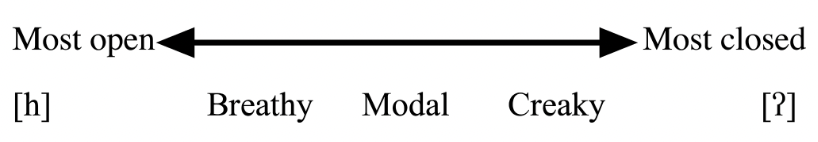
\includegraphics[width=.6\textwidth]{../Phonation.png}
	\caption{Simplified one-deminsional model for phonation. Based on \citet{ladefogedPreliminariesLinguisticPhonetics1971,gordonPhonationTypesCrosslinguistic2001}}.
	\label{fig:Phonation2}
\end{figure}
\vspace{-2ex}
\begin{itemize}
	\item Because the same organ is responsible for these two different phenomena there is a mismatch in trying to produce both at the same time. 
	\item The LCH assumes that there needs to be a strict ordering in the glottal gestures. 
	\item If the gestures were overlapped there will be a perturbation of the tone and the listeners will not be able to reliably differentiate what the tone is.
	\item The LCH assumes that there is a close link between production and perception. 
	\item This assumption places the responsibility on making sure the acoustic cues are the most perceptually salient on the speaker. 
	\item In Figure~\ref{fig:GlottalGestures}, which is taken from \citet{dicanioCoarticulationToneGlottal2012}, the cue for tone is represented by the Pitch Target and the Glottal Gesture represents the gestures needed to produce phonation. 
\end{itemize}
	\begin{figure}[!ht]
		\centering
		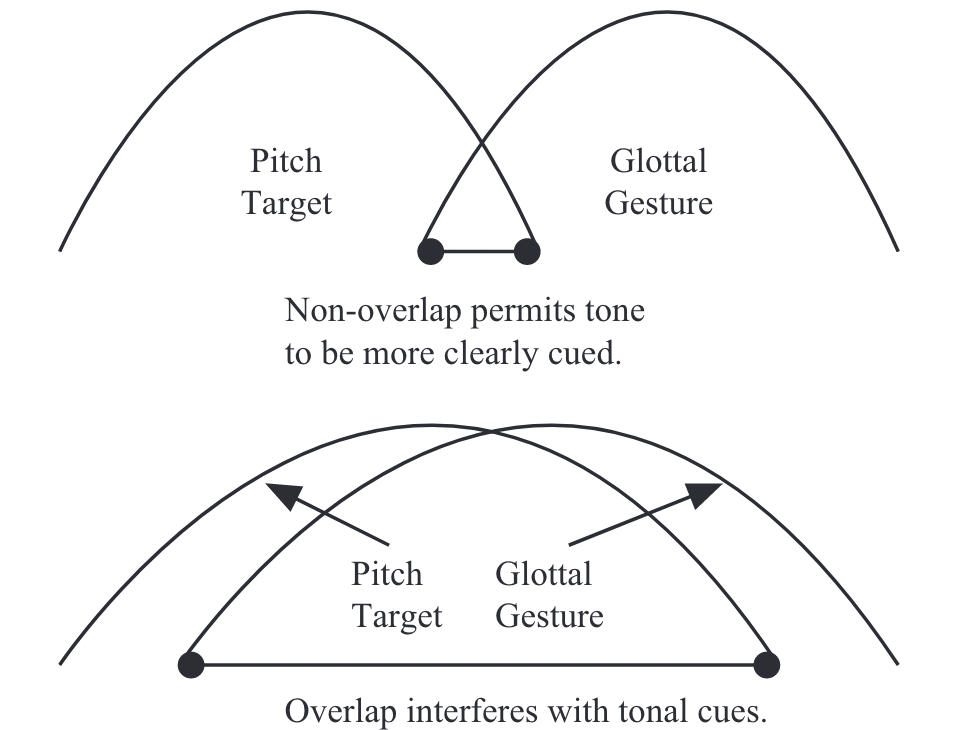
\includegraphics[width=.5\textwidth]{../Gestures.png}
		\caption{Representation taken from \citet{dicanioCoarticulationToneGlottal2012}.}
		\label{fig:GlottalGestures}
	\end{figure}
\begin{itemize}
	\item \citet{dicanioCoarticulationToneGlottal2012} found that when the magnitude of coarticulation for glottal consonants occurs on the vowels there is a strong correlation between the magnitude of overlap and the amount of perturbation in the f0 signal. 
	\item If, however, the degree of overlap was minor then the acoustic signal had little to no perturbation.
	\item Jalapa Mazatec is a language with both contrastive tone and phonation and \citet{garellekAcousticConsequencesPhonation2011} validated the claims made by the LCH, in that tone and phonation seemed to be ordered with each other when it comes to at least one of the phonation types.
	\item SLZ could potentially speak to these differences in timing for nonmodal phonation because of the four way phonation contrast that exists for vowels. 
	\item It already appears from the results of CPP that there is a difference in timing between laryngealized and checked vowels. 
	\item Additionally, SLZ could speak to the phasing of tone and phonation in the vowels, because tone and phonation is orthogonal to one another. 
	\item In order to test the LCH in SLZ, a more controlled token list is needed as well as a larger participant pool to determine if the differences we observe between laryngealized and checked vowels are factual. 
\end{itemize}

%------------------------------------
\section{Conclusion} \label{sec:Conclusion}
%------------------------------------

\begin{itemize}
	\item This paper has provided a brief introduction to SLZ's phonation and the other aspects of its sound system. 
	\item This work is important because SLZ is an understudied variety of Northern Zapotec and there is very little about the phonetics or phonology of this language available. 
	\item Additionally, this paper has shown that H1-H2 was not a very reliable measurement for FSR's or RD's phonation type. 
	\item In line with \citet{espositoVariationContrastivePhonation2010}, H1-A3 seemed to be the more reliable phonation type measurement, at least for breathy voice. 
	\item Additionally, CPP was shown to be a very good indicator for checked and laryngealized vowels in SLZ. 
	\item Additionally, CPP seemed to be primarily different in terms of timing for checked and laryngealized. 
	\item This study will benefit from further analysis and data collection. 
	\item Now that the world is in a safer state in regards to COVID-19 it is important to collect data from more speakers to confirm the data and analysis from FSR and RD.
\end{itemize}

%------------------------------------
%\subsection{} \label{}
%------------------------------------

%------------------------------------
%BIBLIOGRAPHY
%------------------------------------

%\singlespacing
% \nocite{*}
\printbibliography[heading=bibintoc]

\end{document} 